%Copyright 2019 Christopher M. Jermaine (cmj4@rice.edu) and Risa B. Myers (rbm2@rice.edu)
%
%Licensed under the Apache License, Version 2.0 (the "License");
%you may not use this file except in compliance with the License.
%You may obtain a copy of the License at
%
%    https://www.apache.org/licenses/LICENSE-2.0
%
%Unless required by applicable law or agreed to in writing, software
%distributed under the License is distributed on an "AS IS" BASIS,
%WITHOUT WARRANTIES OR CONDITIONS OF ANY KIND, either express or implied.
%See the License for the specific language governing permissions and
%limitations under the License.
%===============================================================
\documentclass[aspectratio=169]{beamer}
\mode<presentation> 
{
\usetheme[noshadow, minimal,numbers,riceb,nonav]{Rice}
\usefonttheme[onlymath]{serif}
\setbeamercovered{transparent}
}
\useinnertheme{rectangles}

\usepackage[english]{babel}

\usepackage{mathptmx}
\usepackage{helvet}
\usepackage{courier}
\usepackage[T1]{fontenc}
\usepackage{trajan}

\setbeamerfont{block body}{size=\tiny}
\usepackage{listings}

%===============================================================%
\title[]
{Tools \& Models for Data Science}

\subtitle{Over-Fitting and Regularization}

\author[]{Chris Jermaine \& Risa Myers}
\institute
{
  Rice University
}

\date[]{}

\subject{Beamer}


\begin{document}
\begin{frame}
 \titlepage
\end{frame}

%***********************************************************
\begin{frame}{Over-Fitting}

\begin{itemize}
	\item Fundamental problem in data science
        \begin{itemize}
                \item Given enough hypotheses to check...
		\item One of them is bound to be true
        \end{itemize}
\end{itemize}
\end{frame}
%***********************************************************
\begin{frame}{Miss America and Murder-By-Steam}

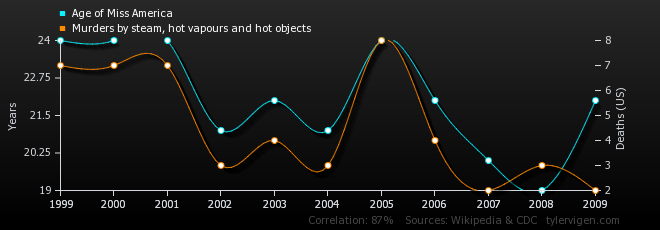
\includegraphics[width=0.9\textwidth]{lectReg/age-of-miss-america_murders-by-steam-hot-vapours-and-hot-objects.png}
\footnote{\url{http://tylervigen.com/view_correlation?id=2948}}
\end{frame}

%***********************************************************
\begin{frame}{Predicting the S\&P 500}

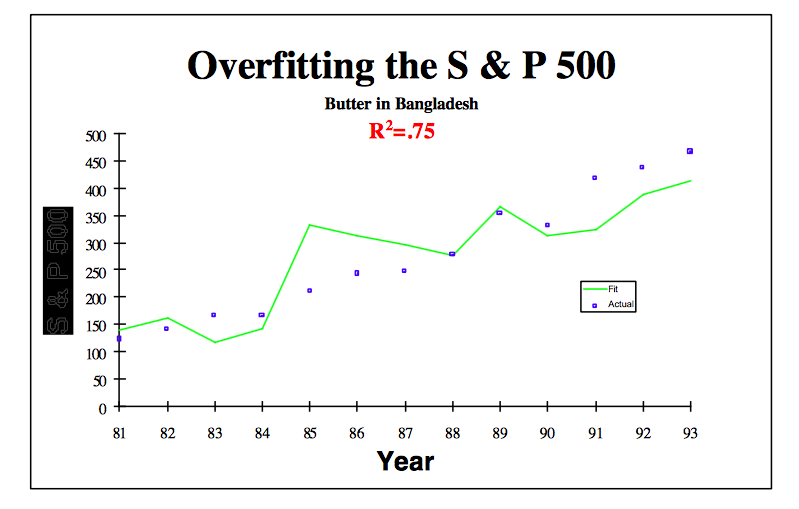
\includegraphics[width=0.7\textwidth]{./lectReg/butter1.png}
\footnote{\url{Leinweber DJ. Stupid data miner tricks: overfitting the S&P 500. Journal of Investing. 2007;16(1):15.
}}
\end{frame}

%***********************************************************
\begin{frame}{Predicting the S\&P 500}

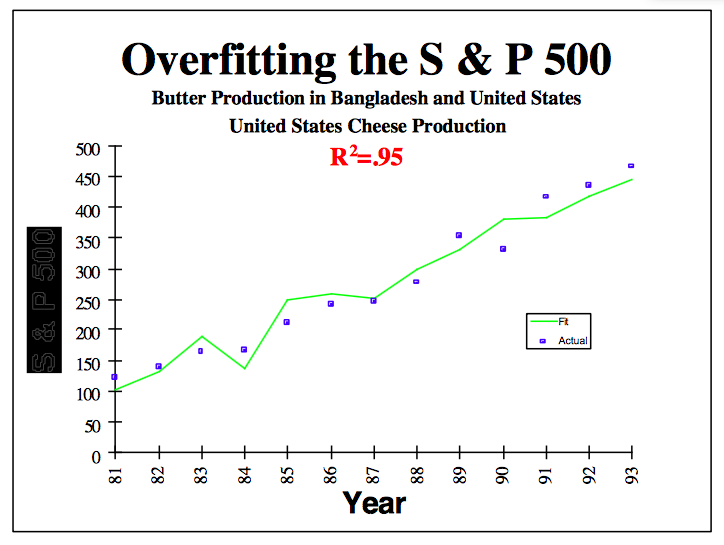
\includegraphics[width=0.65\textwidth]{./lectReg/butter2.png}
\footnote{\url{Leinweber DJ. Stupid data miner tricks: overfitting the S&P 500. Journal of Investing. 2007;16(1):15.
}}
\end{frame}

%***********************************************************
\begin{frame}{Predicting the S\&P 500}

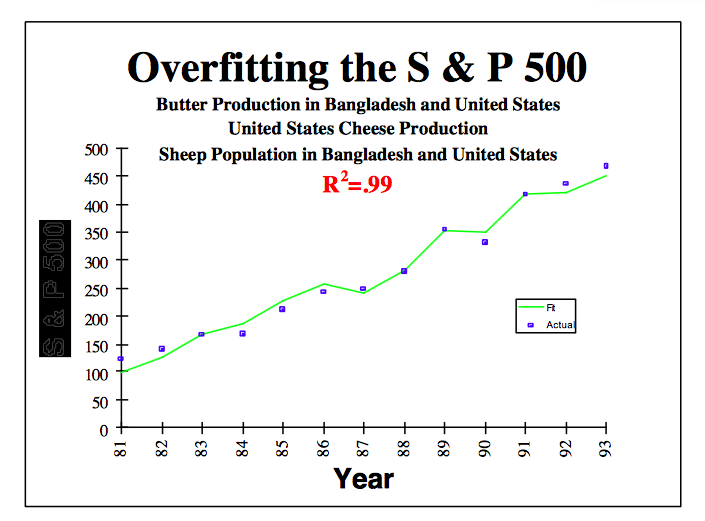
\includegraphics[width=0.65\textwidth]{./lectReg/butter3.png}
\footnote{\url{Leinweber DJ. Stupid data miner tricks: overfitting the S&P 500. Journal of Investing. 2007;16(1):15.
}}
\end{frame}
%***********************************************************
\begin{frame}{Fishing and the S\&P 500}

\begin{columns}[T]
\begin{column}{0.2\textwidth}
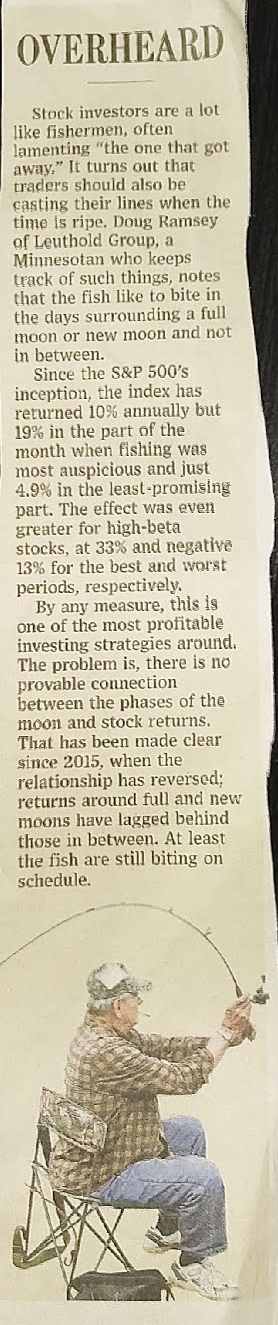
\includegraphics[width=.7\textwidth]{lectReg/fishing.jpg}
\end{column}
\begin{column}{0.7\textwidth}

{\tiny

"Since the S\&P 500's inception, the index has returned 10.3\% annually but 19\% in the part of the month when fishing was most auspicious and just 4.9\% in the least-promising part. The effect was even greater for high-beta stocks at 33.4\% and negative 13.4\% for the best and worst periods, respectively."\\

"By any measure this is one of the most profitable investing strategies around. The problem is, there is no provable connection between the phases of the moon and stock returns. That has been made clear since 2015, when the relationship has reversed--returns around full and new moons have lagged those in between. At least the fish are still biting on schedule."\footnote{https://blogs.wsj.com/moneybeat/2018/06/01/this-trading-strategy-is-the-reel-deal/}}


\end{column}
\end{columns}

\end{frame}

%***********************************************************

\begin{frame}{None of these Models Likely to Generalize}

\begin{itemize}
\item That means:
	\begin{itemize}
	\item They've learned the input data
	\item Not any underlying truth
	\item When deployed in the field, likely to fail
	\end{itemize}
\end{itemize}
\end{frame}

%***********************************************************

\begin{frame}{``Data Mining''}

\begin{itemize}
\item Was originally a derogatory term used by stats
	\begin{itemize}
	\item Meant that you could always find something if you look hard enough
	% p-hacking
	\end{itemize}
\end{itemize}
\hspace{6em}
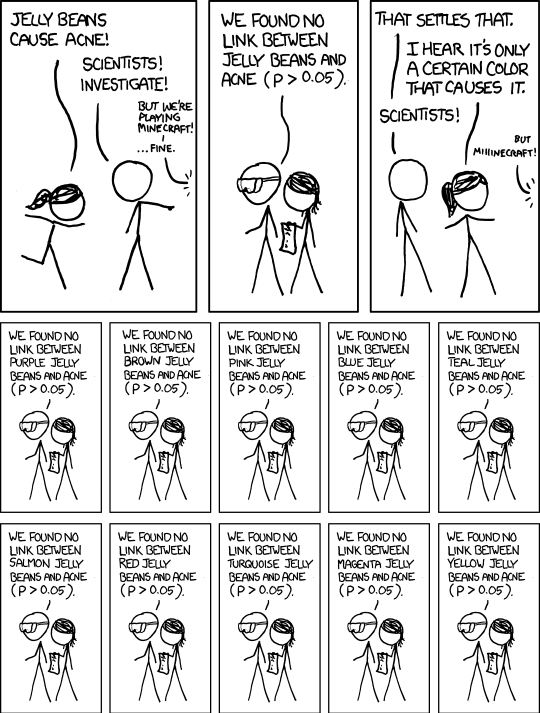
\includegraphics[width=0.3\textwidth]{./lectReg/significant1.png}
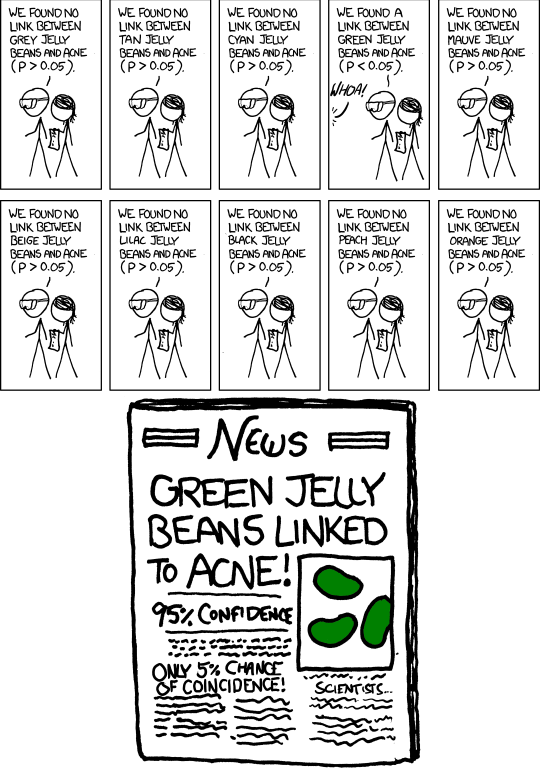
\includegraphics[width=0.3\textwidth]{./lectReg/significant2.png}\footnote{\url{ https://xkcd.com/882/}}
\end{frame}

%***********************************************************

\begin{frame}{Detecting Over-Fitting}

\begin{itemize}
\item Detection method number 1: sniff test 
	\begin{itemize}
	\item E.g.: do the regression coefficients make sense?
	\end{itemize}
\item Detection method number 2: independent validation and test sets
	\begin{itemize}
	\item Avoid temptation!
	\end{itemize}
\item Detection is important...
	\begin{itemize}
	\item Avoiding altogether is as well!
	\end{itemize}
\end{itemize}
\end{frame}
%***********************************************************

\begin{frame}{Sniff Test Example}

\begin{itemize}
\item Predict if patient will be in crisis
\item 4-hour time series epochs
\item 239 patients
\item Researchers started with > 1,000 features
\item Reduced to 50
	\begin{itemize}
	\item including 68th and 143rd most recent observations
	\end{itemize}
\end{itemize}
    	{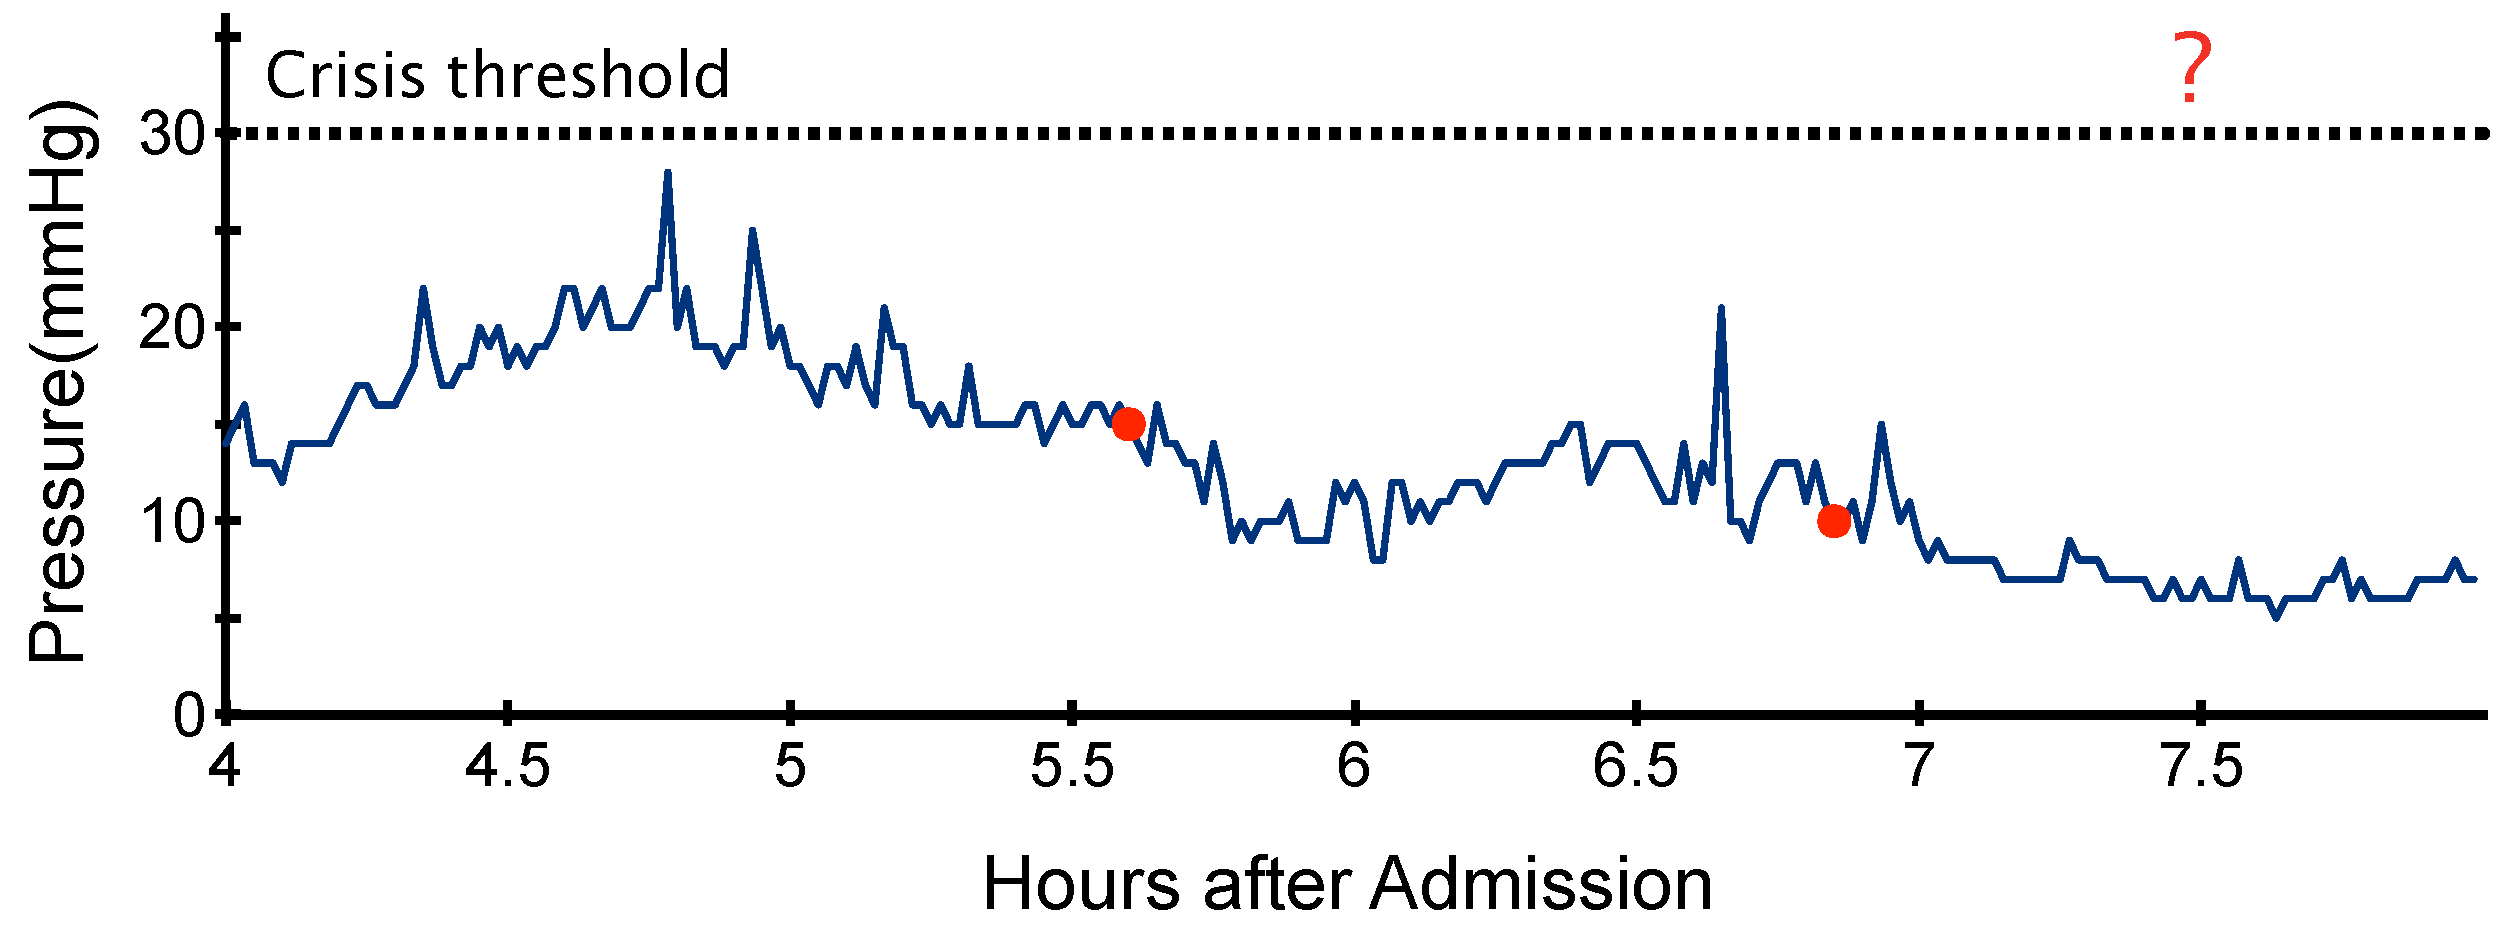
\includegraphics[height=8em]{./lectReg/2102forGuizaOverfit.pdf}} 
	%guiza paper
%***********************************************************
%
%\begin{frame}{Another Sniff Test Example}
%
%\begin{itemize}
%\item Histogram of patient age in a data set
%\item Indicated more likely to visit ER if very young or very old
%\item Sounds fine execpt
%	\begin{itemize}
%	\item It was an adult ER
%	\item Age 0 was used for unknown age
%	\end{itemize}
%\end{itemize}
% What you see is not what you get! Detecting Simpson?s Paradoxes during Data Exploration Yue Guo
\end{frame}
	
%***********************************************************
\begin{frame}{Avoiding Over-Fitting: Occam's Razor}

\begin{itemize}
\item The Razor stated simply: When you have many hypotheses that match observed facts equally well, the simplest one is preferred.
	\begin{itemize}
	\item Been around for a long time!
	\item Credited to William of Ockham (died 1347)
	\item First stated explicitly by John Punch, 1639: ``Entities must not be multiplied beyond necessity''
	\end{itemize}

\end{itemize}
\end{frame}
%***********************************************************

\begin{frame}{Avoiding Over-Fitting: Occam's Razor}

\begin{itemize}
\item Of course, it's not that simple
	\begin{itemize}
	\item You never have a large number of equally good hypotheses
	\item Best you can do: have a preference towards simple models...
	\item Under the assumption they will generalize well
	\end{itemize}
\end{itemize}
\end{frame}


%***********************************************************

\begin{frame}{Occam's Razor Example}

\begin{itemize}
\item Example:
	\begin{itemize}
	\item What's the next number in this sequence?
	\item 1, 3, 5, 7, ?
	\end{itemize}

\end{itemize}
\end{frame}


%***********************************************************
\begin{frame}{Overly Complex Sequence}

\begin{itemize}
	\item 1, 3, 5, 7, ?
	\begin{itemize}
	\item 9\\
\begin{tabular}{lr}
	$$ f(x) = x + 2$$
\end{tabular}
\end{itemize}
\end{itemize}
\end{frame}
%***********************************************************
\begin{frame}{Overly Complex Sequence}

\begin{itemize}
	\item 1, 3, 5, 7, ?
	\begin{itemize}
	\item 217341\footnote{https://ml.berkeley.edu/blog/2017/07/13/tutorial-4/}\\
$$f(x) = \frac{18111}{2} x^4 - 90555x^3 + \frac{633885}{2}x^2 - 452773x + 217331 $$
	\end{itemize}
\end{itemize}
\end{frame}

%***********************************************************

\begin{frame}{Avoiding Over-Fitting: Example Data}

\vspace{1em}
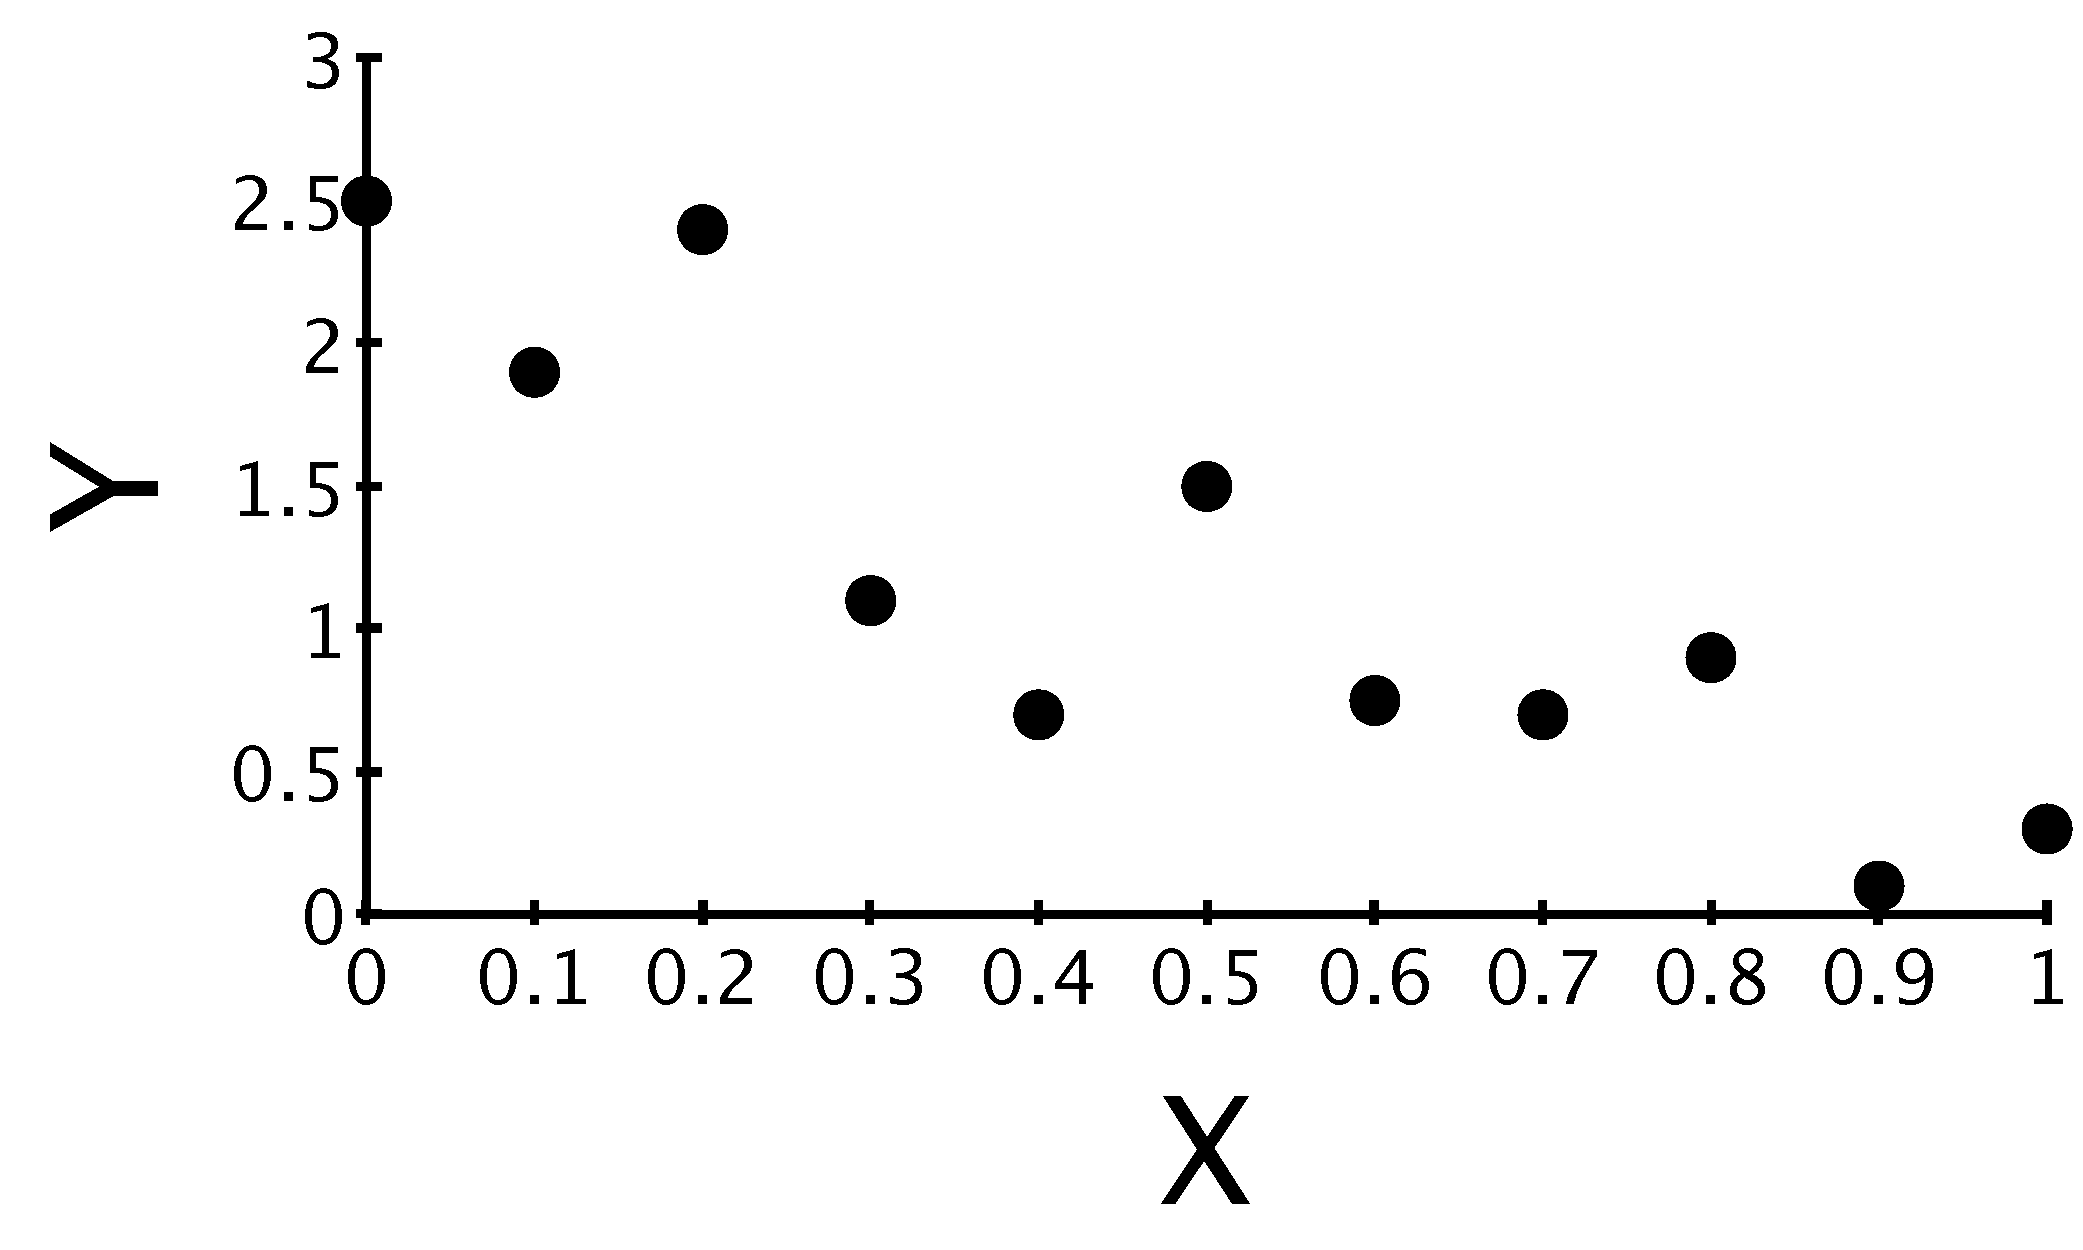
\includegraphics[height=15em]{./lectReg/overfitEx1.pdf}
\end{frame}

%***********************************************************

\begin{frame}{Avoiding Over-Fitting: Example Linear Regression}

\vspace{1em}
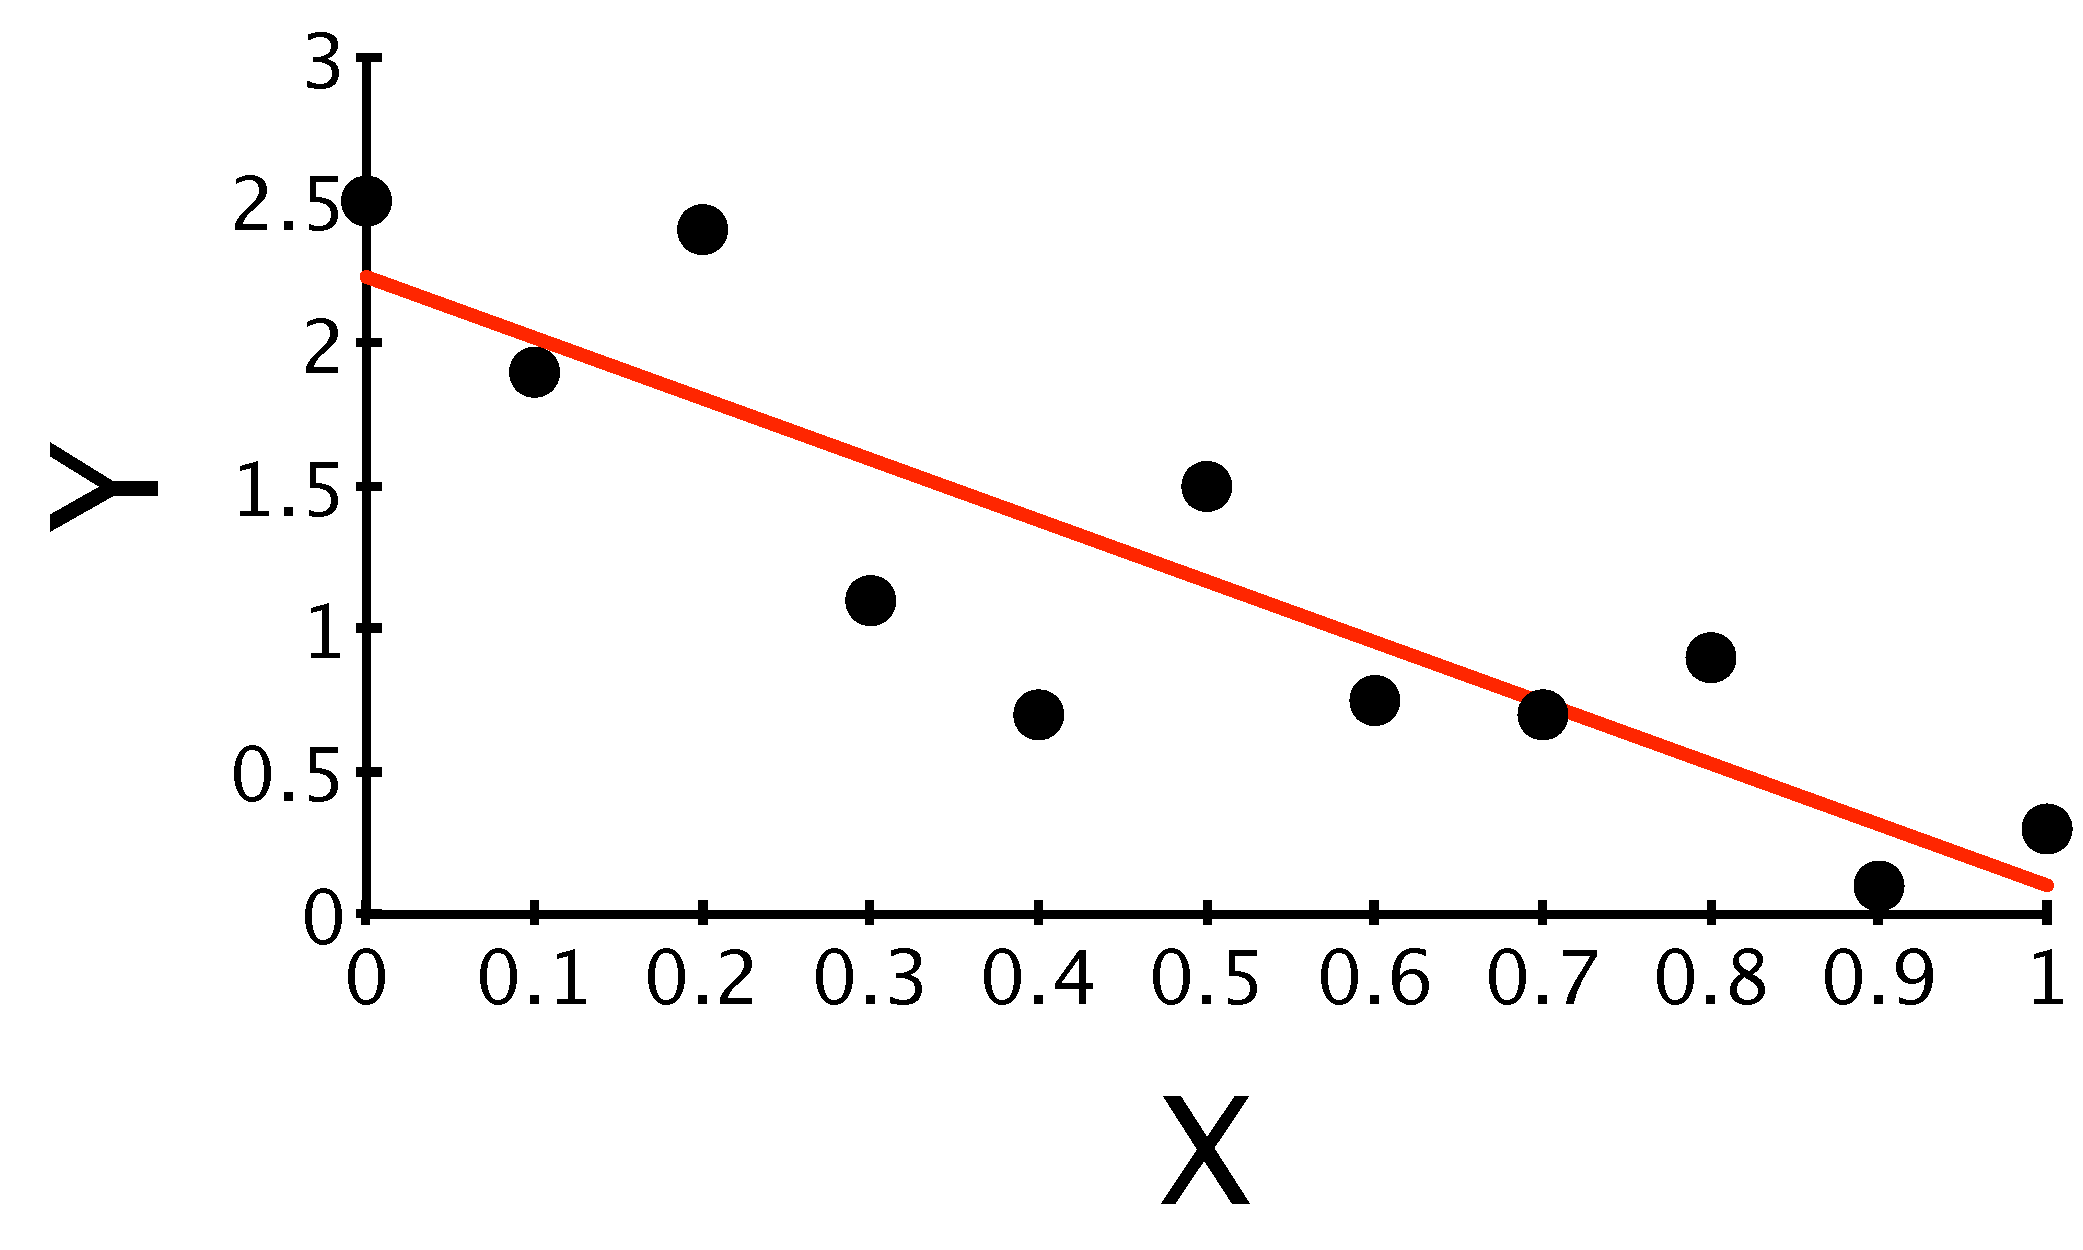
\includegraphics[height=15em]{./lectReg/overfitEx2.pdf}
\end{frame}

%***********************************************************

\begin{frame}{Avoiding Over-Fitting: Example Over-fitting}

\vspace{1em}
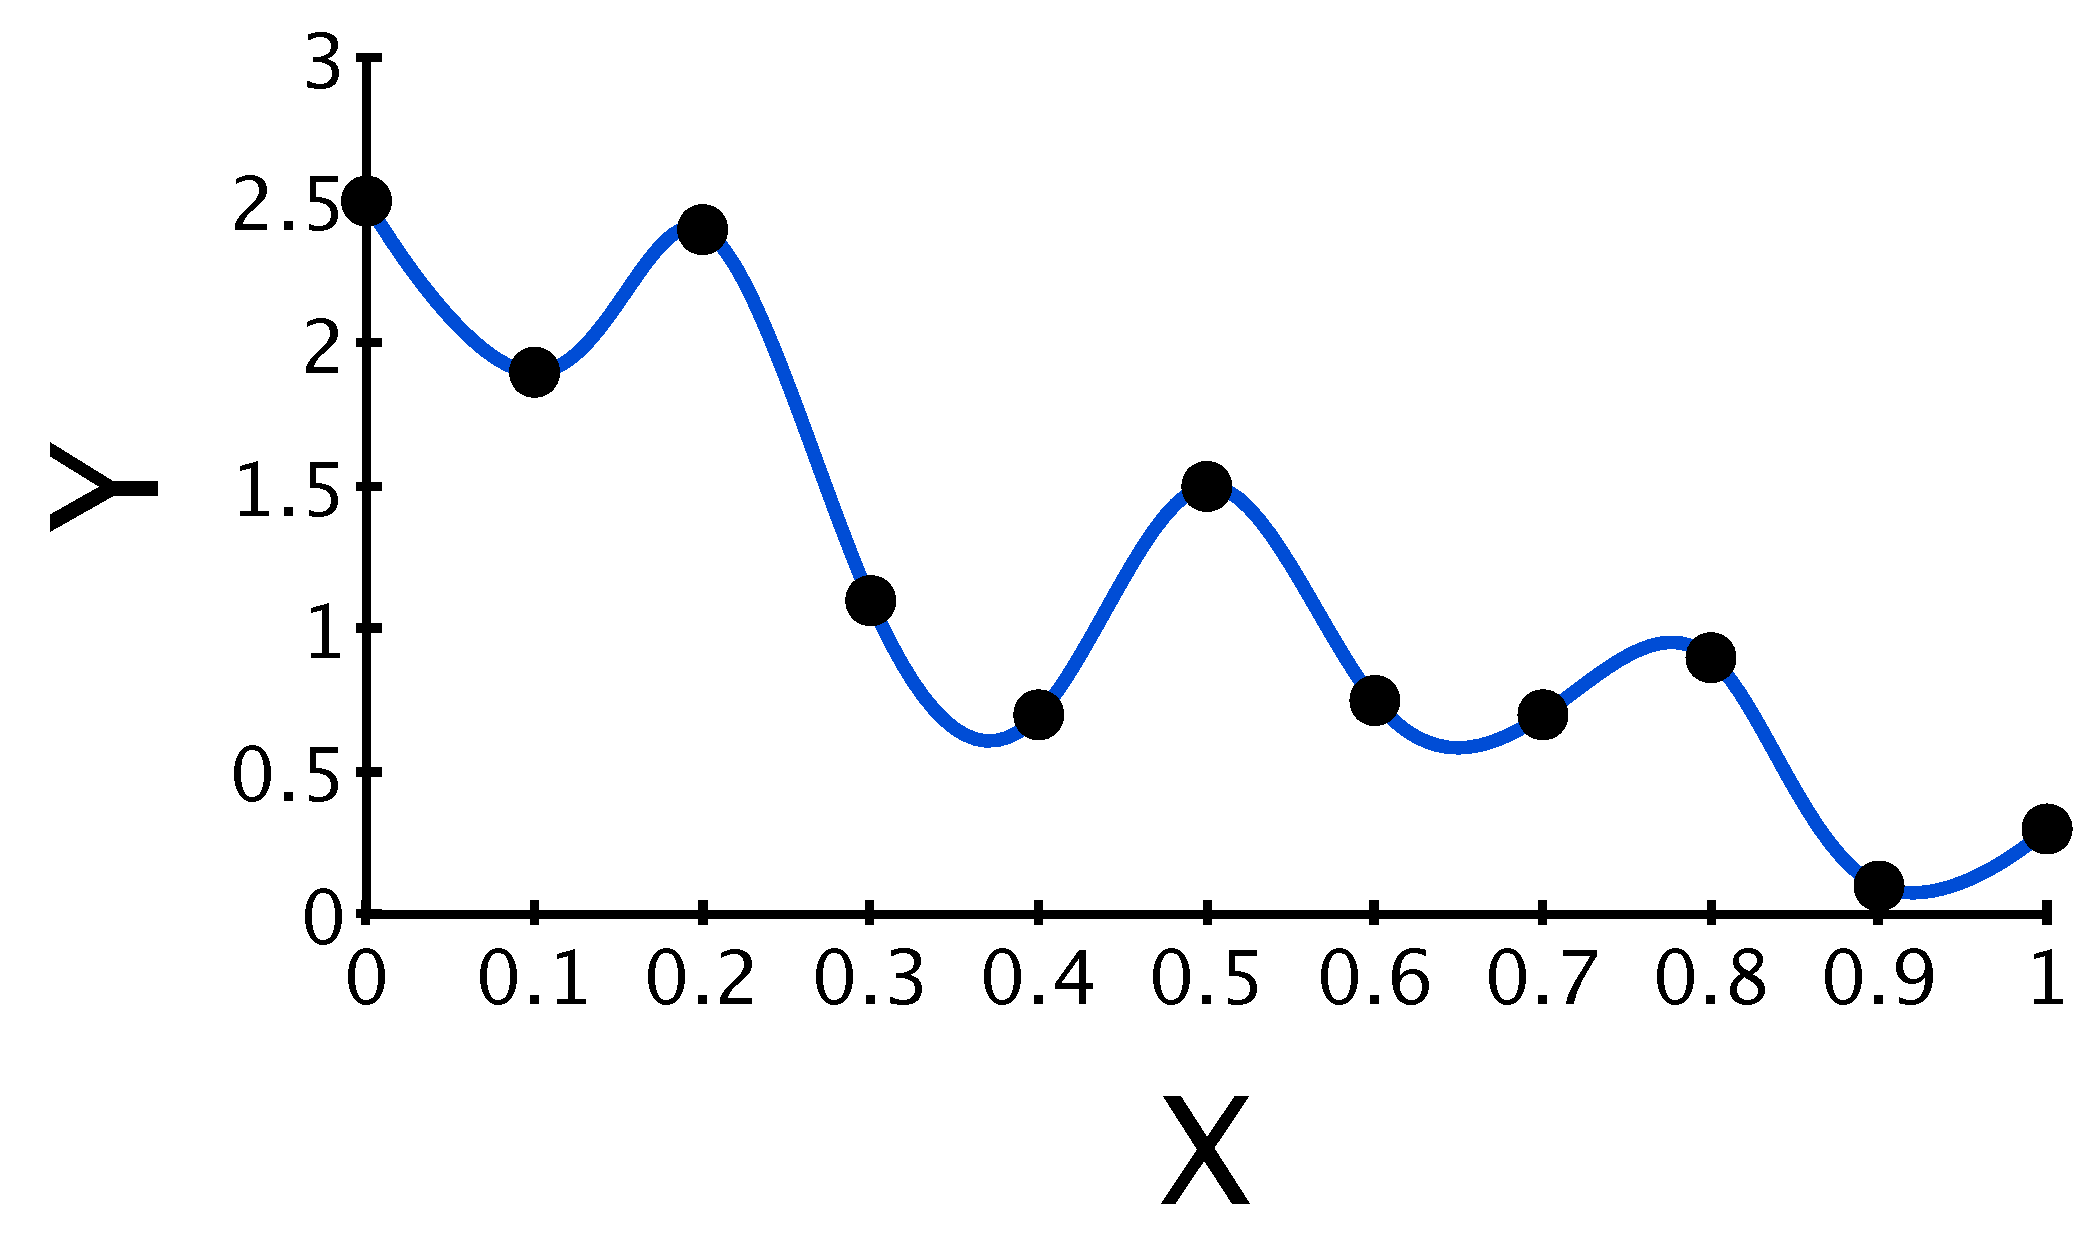
\includegraphics[height=15em]{./lectReg/overfitEx3.pdf}

\end{frame}

%***********************************************************

\begin{frame}{Avoiding Over-Fitting: Example New Point}

\vspace{1em}
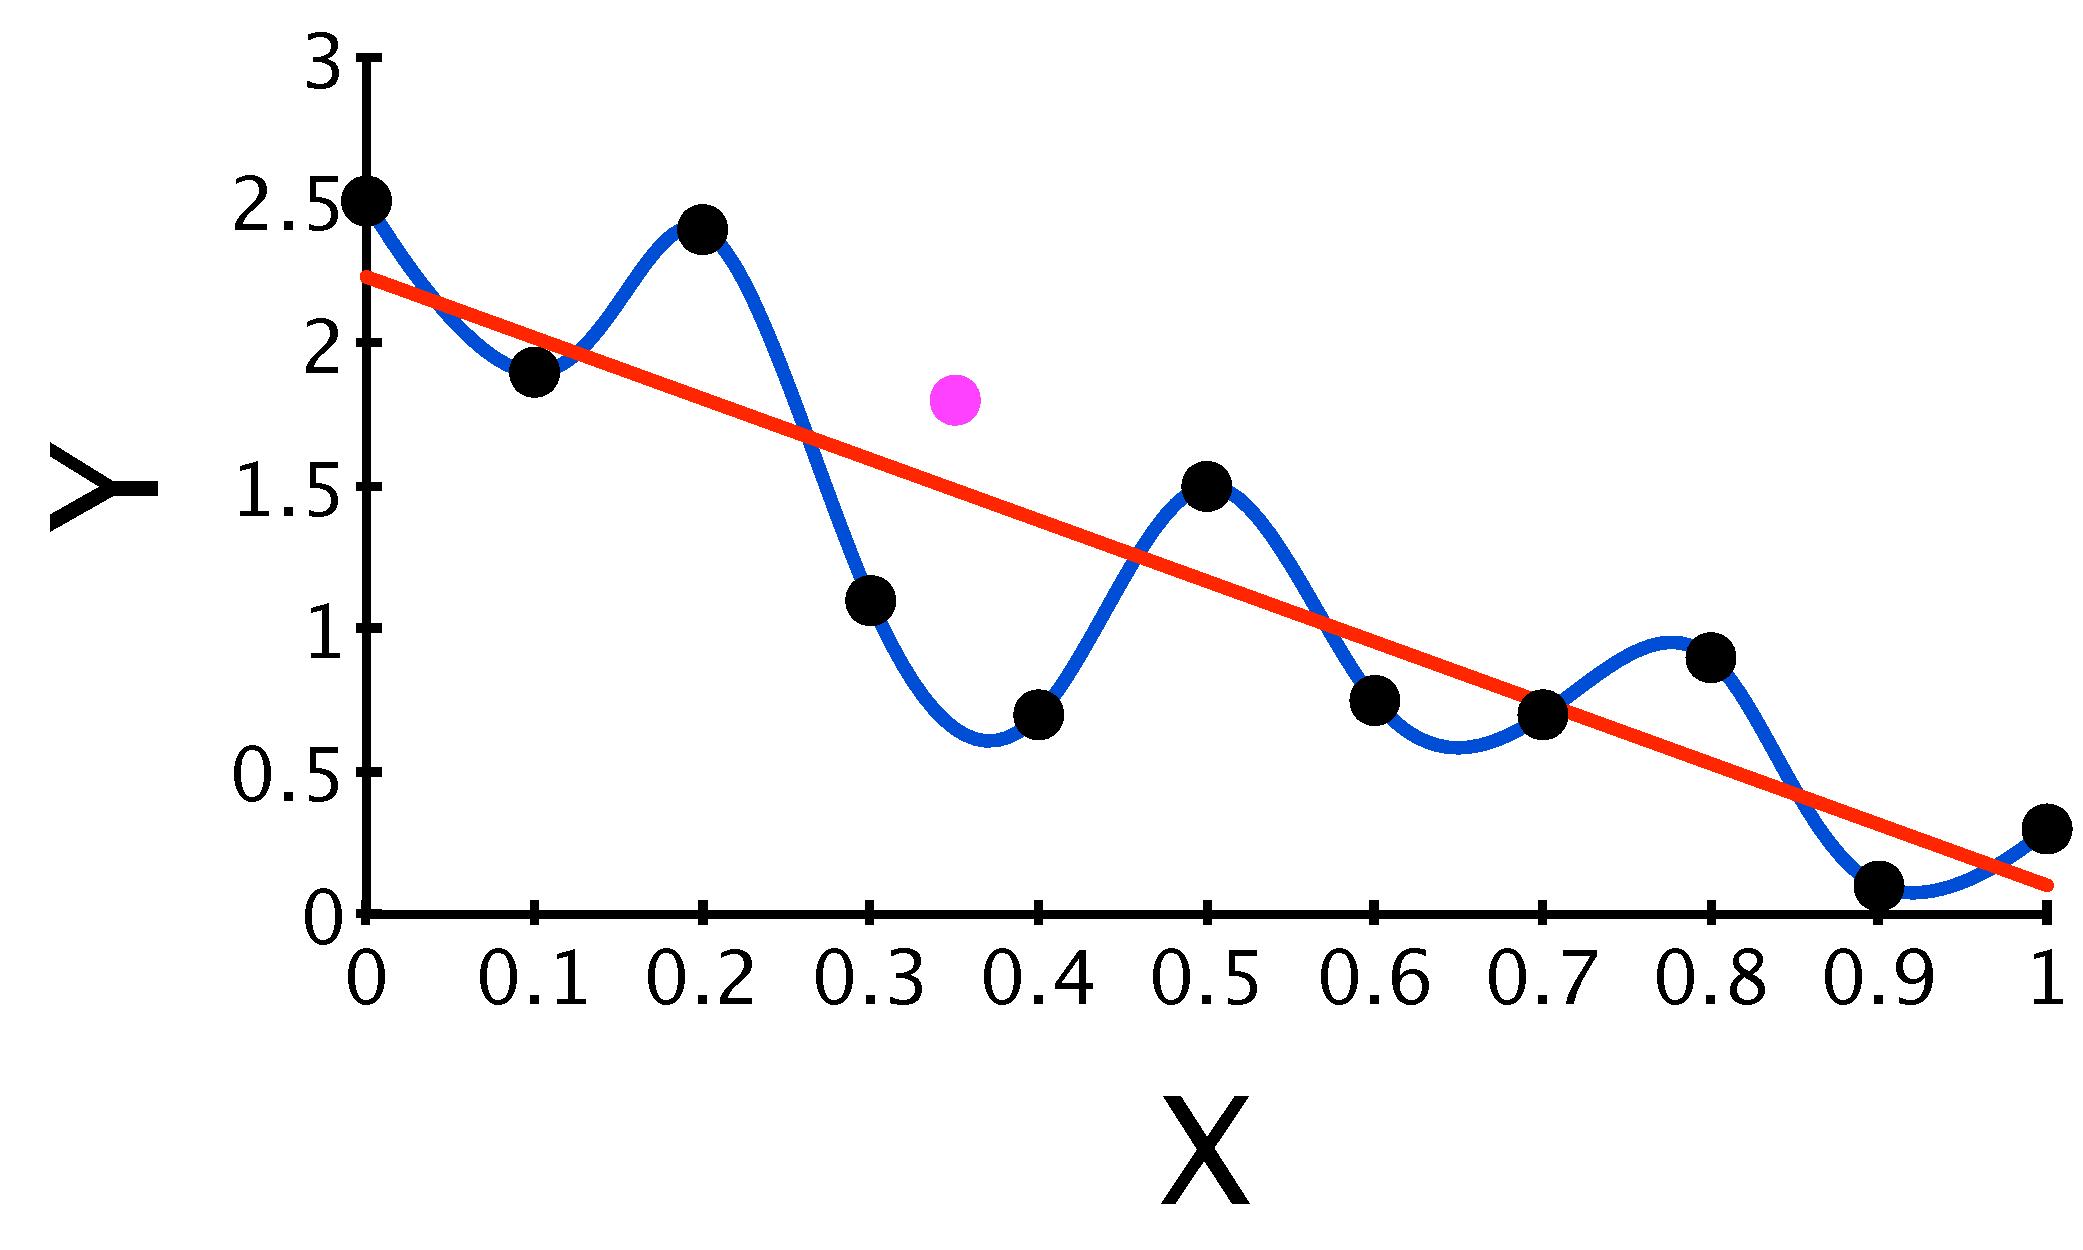
\includegraphics[height=15em]{./lectReg/overfitEx4.pdf}
\end{frame}

%***********************************************************

\begin{frame}{Avoiding Under-Fitting: Example Data}

\vspace{1em}
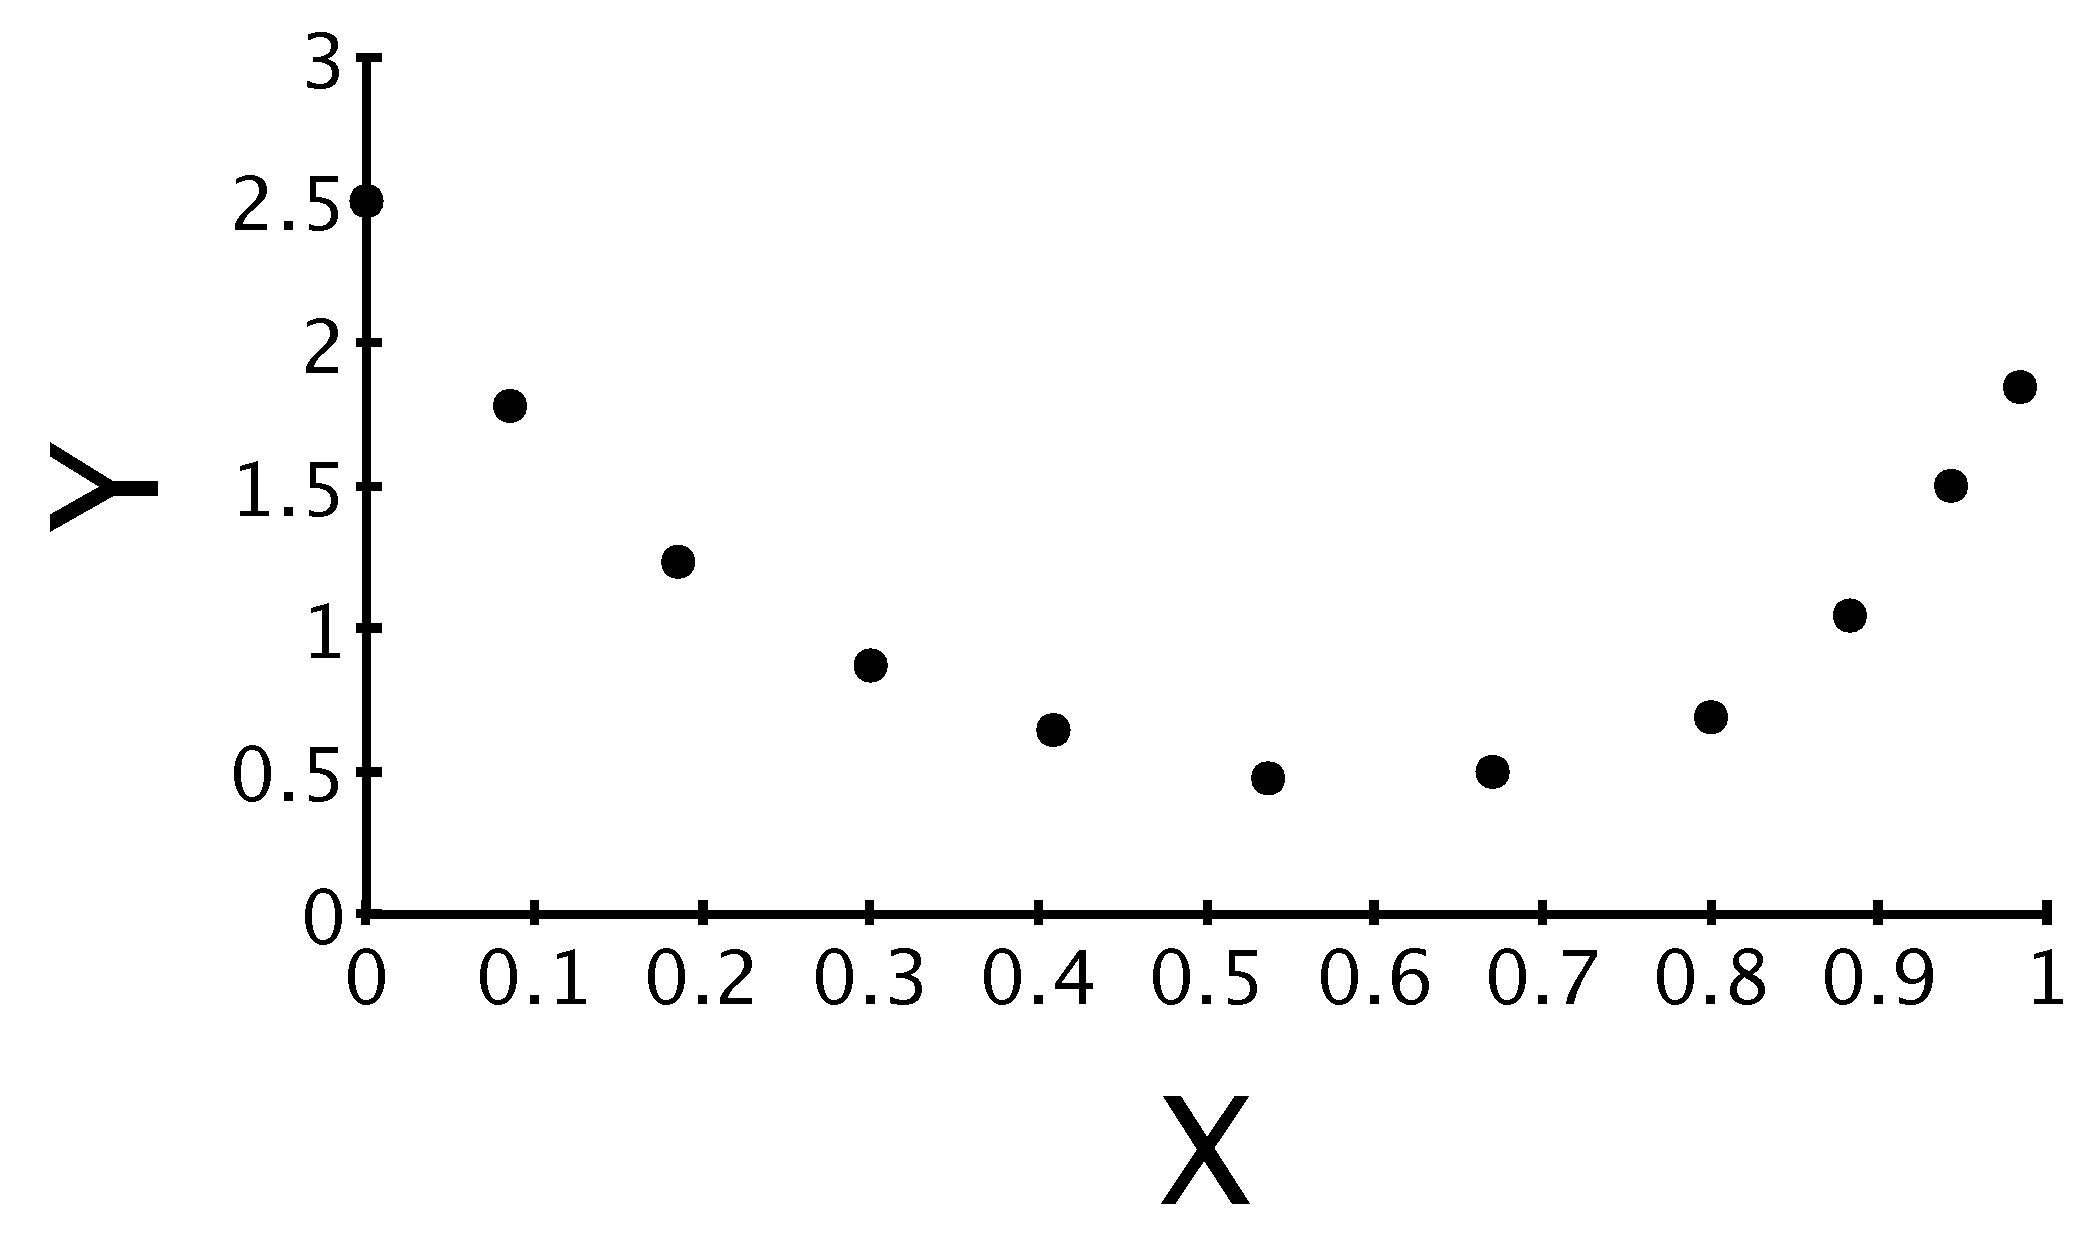
\includegraphics[height=15em]{./lectReg/OverUnderData2.pdf}
\end{frame}
%***********************************************************

\begin{frame}{Avoiding Under-Fitting: Example Under-fitting}

\vspace{1em}
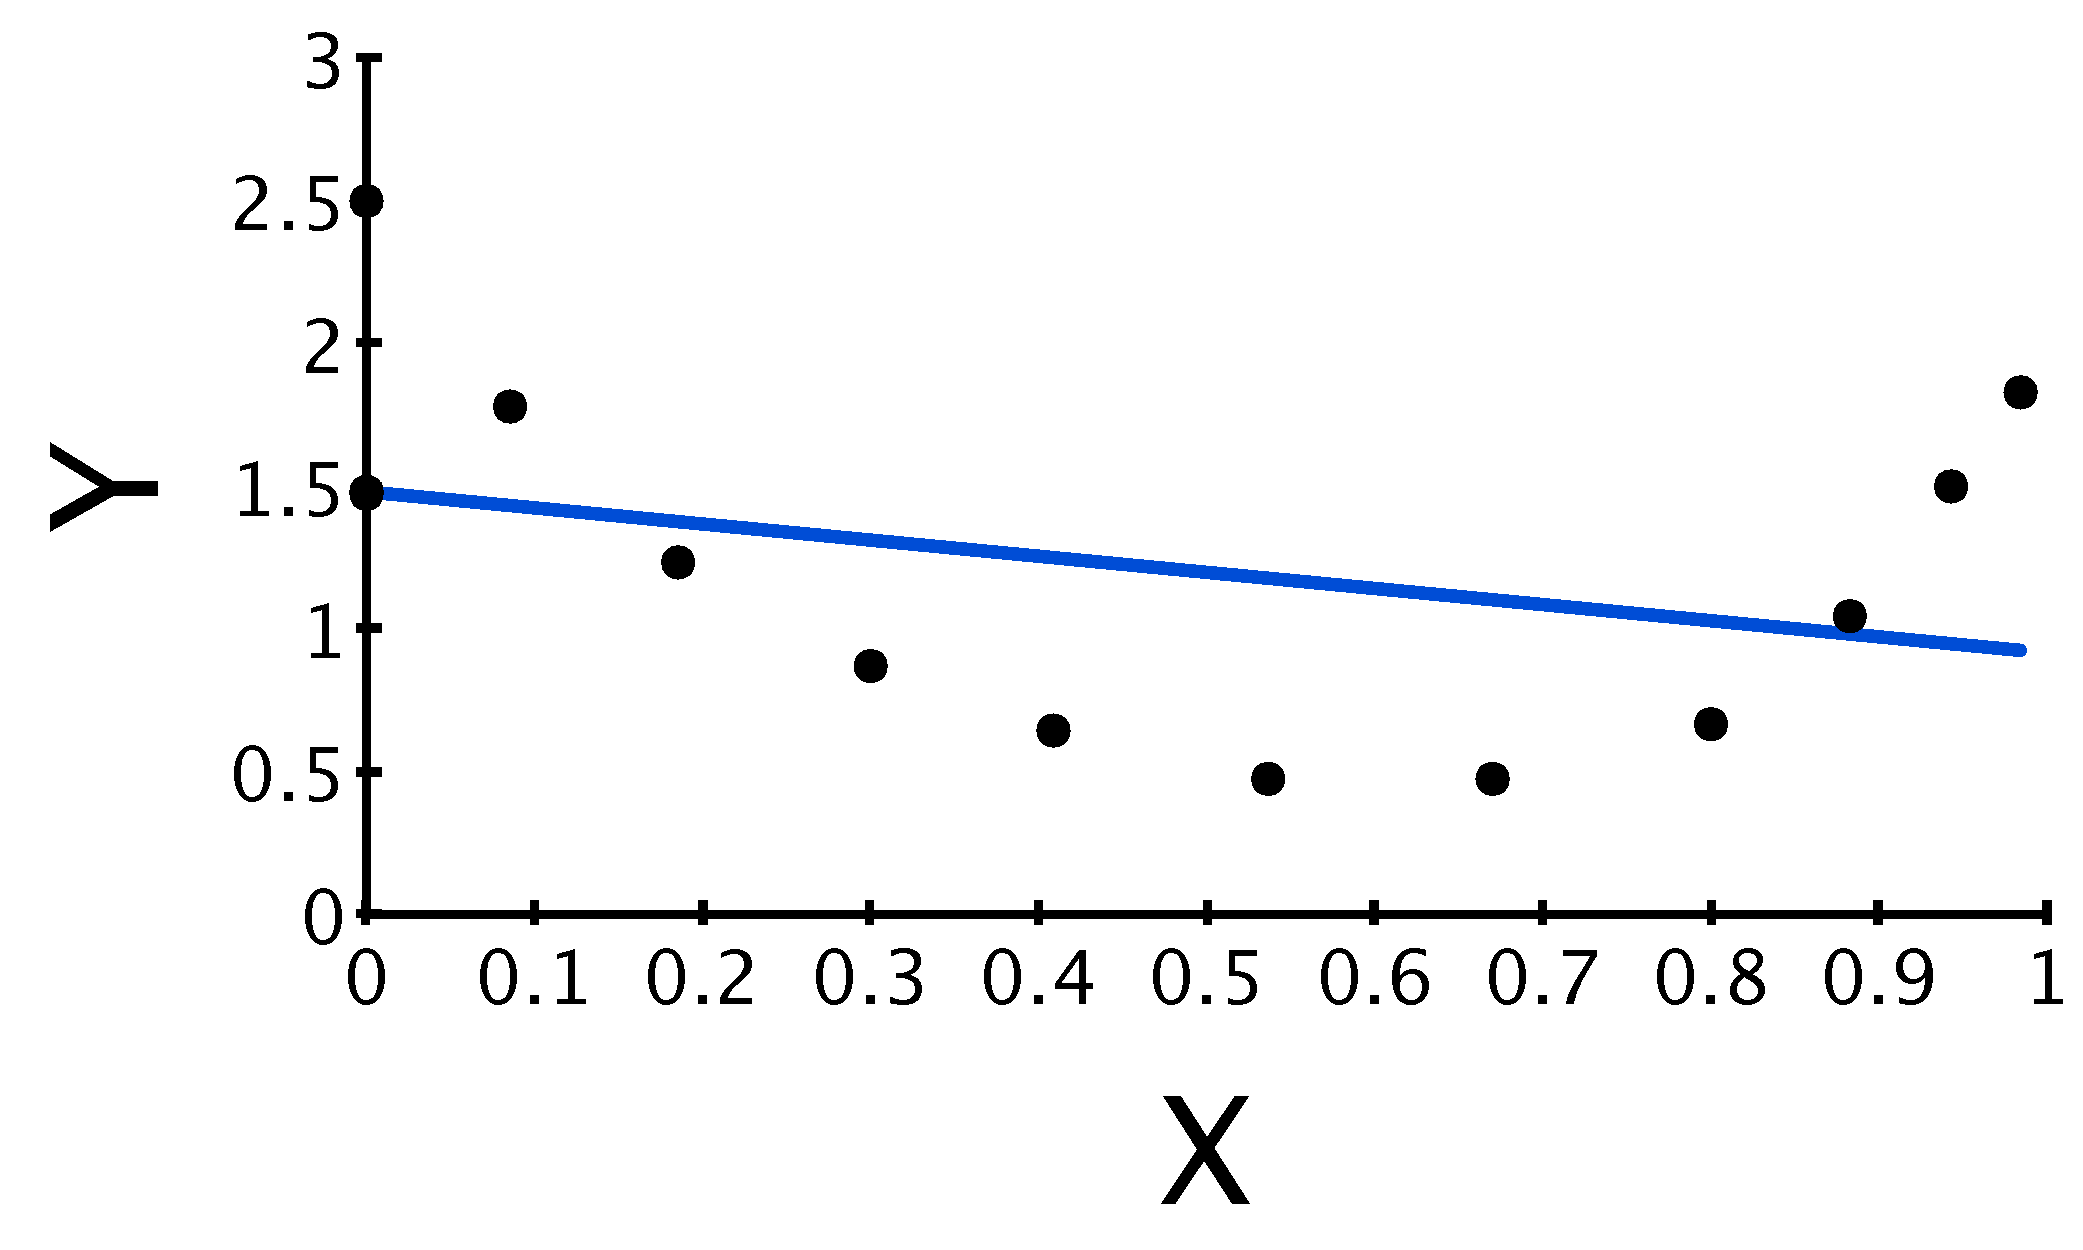
\includegraphics[height=15em]{./lectReg/OverUnderDataU2.pdf}
\end{frame}
%***********************************************************

\begin{frame}{Avoiding Under-Fitting: Example Fitting}

\vspace{1em}
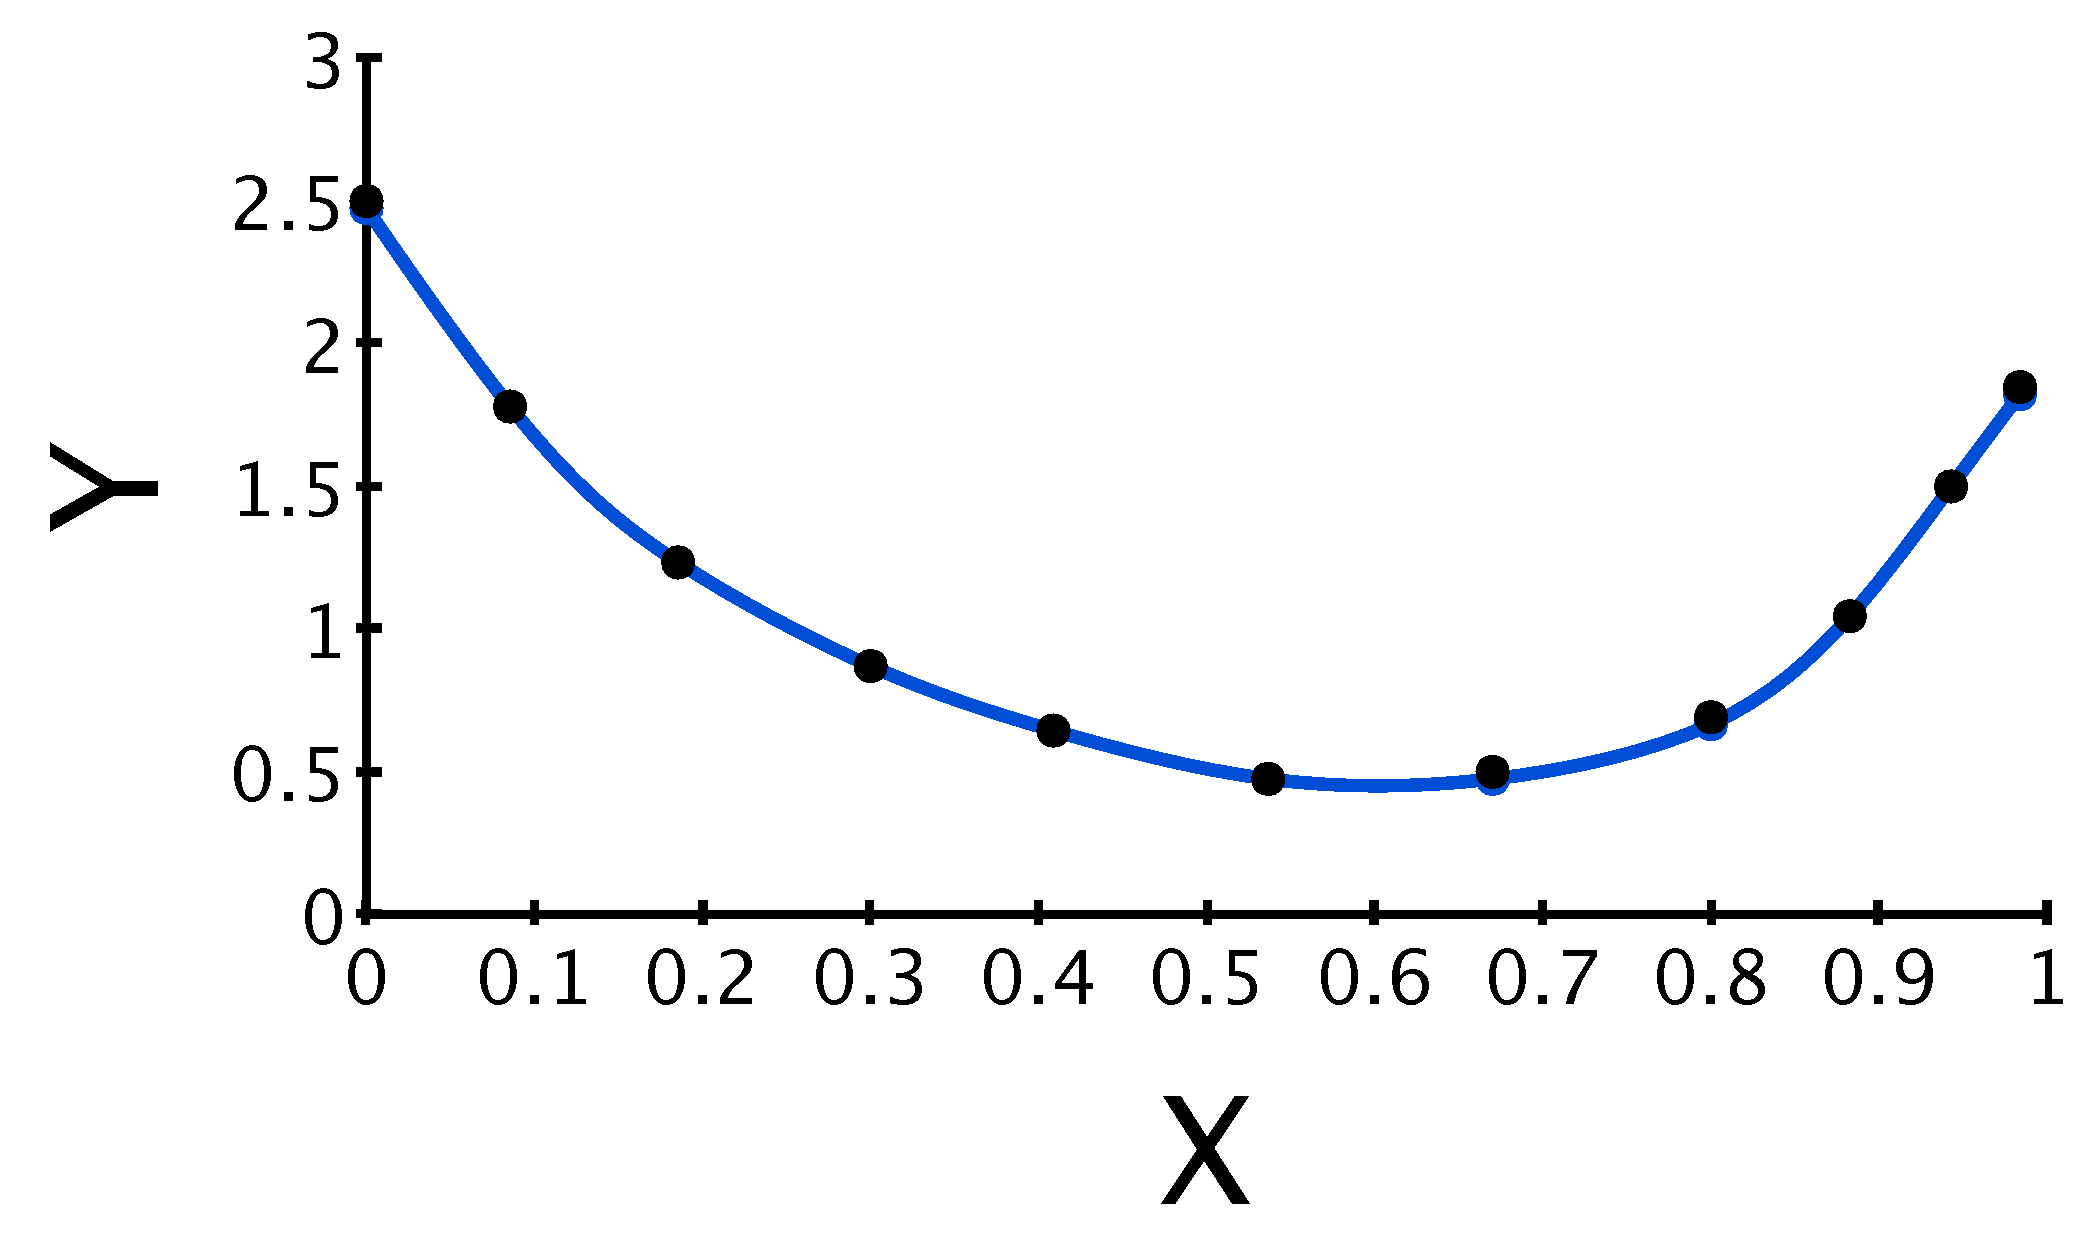
\includegraphics[height=15em]{./lectReg/OverUnderDataFit2.pdf}
\end{frame}

%***********************************************************

\begin{frame}{The Bias-Variance Trade-Off}

\begin{columns}
\begin{column}{0.5\textwidth}
\begin{itemize}
\item In a nutshell, we have two main sources of error in supervised learning
	\begin{itemize}
	\item ``Bias'': error from incorrect model assumptions
	\item ``Variance'': sensitivity of model to bad data
	\end{itemize}
\end{itemize}
\end{column}
\begin{column}{0.5\textwidth}
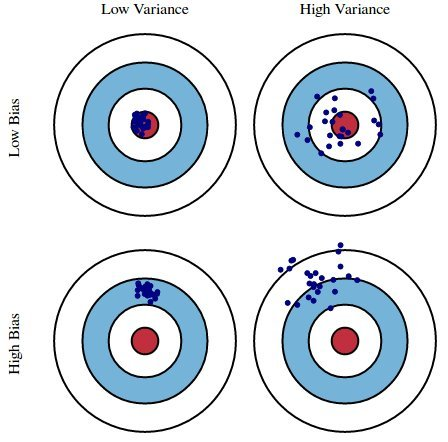
\includegraphics[width=1\textwidth]{./lectReg/bias-and-variance.jpg}
\footnote{\url{http://scott.fortmann-roe.com/docs/BiasVariance.html}}
\end{column}
\end{columns}

%Scott Fortmann-Roe
%http://scott.fortmann-roe.com/docs/BiasVariance.html

\end{frame}

%***********************************************************
\begin{frame}{What is Bias?}

\begin{columns}
\begin{column}{0.5\textwidth}
\begin{itemize}
\item Difference between what our model predicts and the truth
\item Imperfect models
	\begin{itemize}
	\item Simplifying assumptions to make the model easier to learn
	\item What are common simplifying assumptions? 
	% independence of data, the data are linear
	\end{itemize}
%\item If we build multiple models, use the average prediction
%	\begin{itemize}
%	\item Use different data 
%	\item Learn a different model
%	\item When might we build multiple, similar models?
%	% e.g. cross validation
%	\end{itemize}
%\item Each model generates one hit on the target
\end{itemize}
\end{column}
\begin{column}{0.5\textwidth}
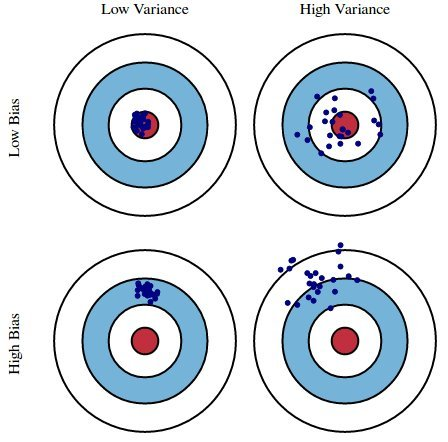
\includegraphics[width=1\textwidth]{./lectReg/bias-and-variance.jpg}
\footnote{\url{http://scott.fortmann-roe.com/docs/BiasVariance.html}}
\end{column}
\end{columns}

\end{frame}
%***********************************************************
\begin{frame}{What is Bias?}

\begin{columns}
\begin{column}{0.5\textwidth}
\begin{itemize}
\item Difference between what our model predicts and the truth
\item Imperfect models
	\begin{itemize}
	\item Simplifying assumptions to make the model easier to learn
	\item What are common simplifying assumptions? 
	\begin{itemize}
	\item iid data 
	\item data distributed normally 
	\end{itemize}
	\end{itemize}
%\item If we build multiple models, use the average prediction
%	\begin{itemize}
%	\item Use different data 
%	\item Learn a different model
%	\item When might we build multiple, similar models?
%	% e.g. cross validation
%	\end{itemize}
%\item Each model generates one hit on the target
\end{itemize}
\end{column}
\begin{column}{0.5\textwidth}
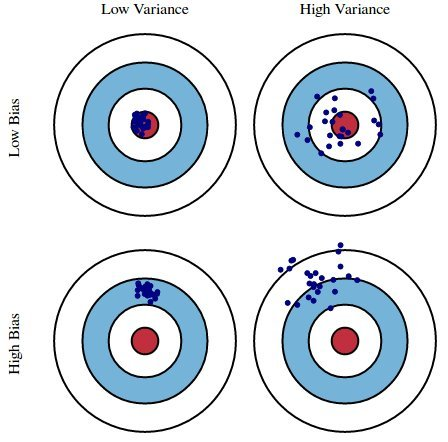
\includegraphics[width=1\textwidth]{./lectReg/bias-and-variance.jpg}
\footnote{\url{http://scott.fortmann-roe.com/docs/BiasVariance.html}}
\end{column}
\end{columns}

\end{frame}

%***********************************************************

%\begin{frame}{Which models are Low/High Bias?}
%
%\begin{itemize}
%\item Parametric models
%	\begin{itemize}
%	\item Make assumptions about the objective function 
%	\item Fast to learn
%	\item Easier to understand
%	\item May UNDERFIT training data
%	% might miss key characteristics
%	\item Linear Regression, Logistic Regression
%	\item High bias
%	\end{itemize}
%\item Non-parametric models
%	\begin{itemize}
%	\item Make few assumptions about the objective function 
%	\item Can be more complex
%	\item kNN, SVM
%	\item Low bias
%	\end{itemize}
%\end{itemize}
%https://machinelearningmastery.com/gentle-introduction-to-the-bias-variance-trade-off-in-machine-learning/
%***********************************************************

\begin{frame}{What is Variance?}

\begin{columns}
\begin{column}{0.5\textwidth}
\begin{itemize}
\item Variability of a model's prediction for a data point
\item If we build multiple models, how consistent are the predictions across these models?
\item Sensitivity of the output to small fluctuations in the training set
\item The model is highly dependent on our selection of training data
	\begin{itemize}
	\item A good distribution of training data will enable us to predict new data well
	\item If our training data has a lot of outliers or non-standard values, our predictions will be off
	\end{itemize}
\end{itemize}
\end{column}
\begin{column}{0.5\textwidth}
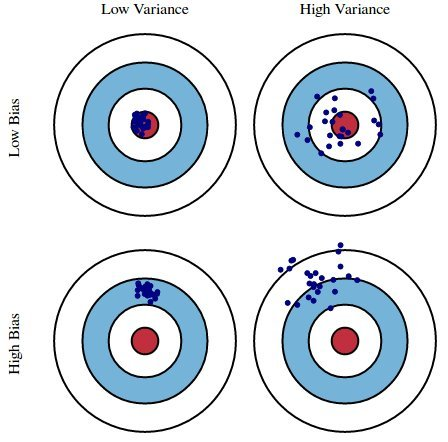
\includegraphics[width=1\textwidth]{./lectReg/bias-and-variance.jpg}
\footnote{\url{http://scott.fortmann-roe.com/docs/BiasVariance.html}}
\end{column}
\end{columns}
\end{frame}

%***********************************************************
\begin{frame}{The Bias-Variance Target}

\begin{columns}
\begin{column}{0.5\textwidth}
\begin{itemize}
\item Suppose we have a number of DIFFERENT training sets for the same problem
\item Train the same algorithm on each of the training sets
\item Each hit on the target is generated by a single model
\item A perfect classifier would hit the bulls-eye
\end{itemize}
\end{column}
\begin{column}{0.5\textwidth}
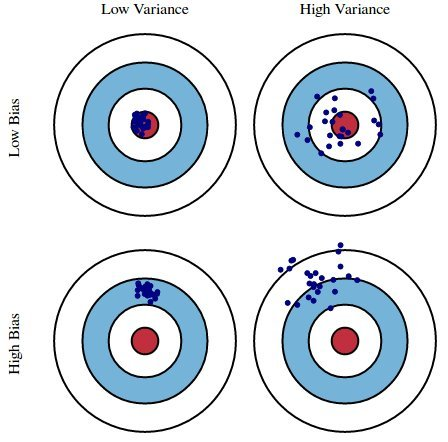
\includegraphics[width=1\textwidth]{./lectReg/bias-and-variance.jpg}
\footnote{\url{http://scott.fortmann-roe.com/docs/BiasVariance.html}}
\end{column}
\end{columns}
\end{frame}

%***********************************************************
\begin{frame}{Understanding the Trade-Off}

\begin{itemize}
\item Expected squared error of any prediction is:
	 $$E[(Y - \hat{f}(X))^2]$$ 
	\begin{itemize}
	\item $Y$ is the value we are trying to predict from X
	\item $\hat{f}(.)$ is the model we are learning (is a random variable!)
	\item $X$ is the observed data (ex: set of regressors)
	\end{itemize}
\end{itemize}
\end{frame}

%***********************************************************
\begin{frame}{Some Definitions}

\begin{itemize}
\item $Var(Y) = E[Y^2] - E^2[Y]$
\item $Bias^2(\hat{f}(x)) = E^2[\hat{f}(x) - Y]$
\end{itemize}
\end{frame}

%***********************************************************
\begin{frame}{Understanding the Trade-Off}

\begin{itemize}
\item Expected squared error of any prediction is $E[(Y - \hat{f}(X))^2]$
	\begin{itemize}
	\item Expanding:
	\begin{align}
	E[(Y - \hat{f}(x))^2] &= E[Y^2 + \hat{f}^2(x) - 2Y\hat{f}(x)] \nonumber \\
			      &= E[Y^2] + E[\hat{f}^2(x)] - E[2Y\hat{f}(x)] \nonumber \\
			      &= Var(Y) + E^2[Y] + E[\hat{f}^2(x)] - E[2Y\hat{f}(x)] \nonumber \\
			      &=  Var(Y) + E^2[Y] + Var(\hat{f}(x)) + E^2[\hat{f}(x)] - E[2Y\hat{f}(x)] \nonumber \\
			      &= Var(Y) + Var(\hat{f}(x)) + (E^2[Y] - E[2Y\hat{f}(x)] + E^2[\hat{f}(x)]) \nonumber \\
			      &= Var(Y) + Var(\hat{f}(x)) + Bias^2(\hat{f}(x)) \nonumber
	\end{align}
	\item Means error is a sum of:
	\item ``Looseness'' of relationship between $X$ and $Y$
	\item Sensitivity of the learner to variability of the training data (variance)
	\item Inability of the learner $\hat{f}$ to learn the relationship between $X$ and $Y$ (bias)
%	\item Var(Y) is irreducible error
	% if I repeat a trial a number of times (job 3 miles every morning
	\end{itemize}
\item It is the second one (variance) that leads to over-fitting
\end{itemize}
\end{frame}
%***********************************************************
\begin{frame}{Understanding the Trade-Off}

\begin{itemize}
\item How did we derive the last step? 
	\begin{itemize}
	\item Note that $Bias(\hat{f}(x)) = E[\hat{f}(x) - Y]$. So:
	\begin{align} 
	Bias^2(\hat{f}(x)) &= E^2[\hat{f}(x) - Y] \nonumber \\
			   &= (E[\hat{f}(x) - Y])(E[\hat{f}(x) - Y]) \nonumber \\
			   &= (E[\hat{f}(x)] - E[Y])(E[\hat{f}(x)] - E[Y]) \nonumber \\
			   &= E^2[Y] - 2E[\hat{f}(x)]E[Y] + E^2[\hat{f}(x)] \nonumber \\
			   &= E^2[Y] - E[2Y\hat{f}(x)] + E^2[\hat{f}(x)] \nonumber
	\end{align}
	\item So
	\begin{align}
		&Var(Y) + Var(\hat{f}(x)) + (E^2[Y] - E[2Y\hat{f}(x)] + E^2[\hat{f}(x)]) \nonumber \\
		&= Var(Y) + Var(\hat{f}(x)) + Bias^2(\hat{f}(x)) \nonumber
	\end{align}
	\end{itemize}
\end{itemize}
\end{frame}

%%***********************************************************
%\begin{frame}{Irreducible Error}
%	\begin{align}
%	E[(Y - \hat{f}(X))^2] &=  Var(Y) + Var(\hat{f}(X)) + Bias^2(\hat{f}(X)) \nonumber
%	\end{align}
%\begin{itemize}
%\item Var(Y) is irreducible error
%	\begin{itemize}
%\item Inherent variability in the outcomes
%\item Noise
%	\end{itemize}
%\end{itemize}
%\end{frame}

%***********************************************************
\begin{frame}{Irreducible Error}

\begin{itemize}
	\item Since we have:
	$$E[(Y - \hat{f}(x))^2] = Var(Y) + Var(\hat{f}(x)) + Bias^2(\hat{f}(x))$$
	\item Means error of supervised learner is a sum of:
	\begin{itemize}
	\item ``Looseness'' of relationship between $x$ and $Y$ ($Var(Y)$)
	\item Sensitivity of the learner to variability of the training data ($Var(\hat{f}(x))$)
	\item Inability of the learner $\hat{f}$ to learn the relationship between $X$ and $Y$ ($Bias^2(\hat{f}(x))$)
	\end{itemize}
\item $\textrm{\textit{It is the sensitivity of the learner to variability of the training data}}$
\item $\textrm{\textit{that leads to over-fitting}}$
\end{itemize}
\end{frame}

		
%***********************************************************
\begin{frame}{Ideally, Reduce Both Bias and Variance!}

\begin{itemize}
\item Unfortunately, not possible
\item ``In real life''...
	\begin{itemize}
	\item Exceedingly general models are a problem
	\item They are difficult to train (lots of local mins, need tons of data)
	\item So you design a model to solve your problem
	\item Lowers $Var(\hat{f}(X))$ (damage due to over-fitting)
	\item But increases so-called ``inductive bias'' (bias introduced in the model you chose)
	\item Best we can do: choose sweet spot where error is minimized
	\item To avoid necessity of high model bias, use methods to avoid over-fitting
	\end{itemize}
\end{itemize}
\end{frame}

%%***********************************************************
%\begin{frame}{Types of Bias in Data}
%
%\begin{itemize}
%\item 
%\item ``In real life''
%	\begin{itemize}
%	\item 
%	\end{itemize}
%\end{itemize}
%\end{frame}



%***********************************************************
%\begin{frame}{Model Complexity vs. Error}
%\vspace{2em}
%\hspace{2em}
%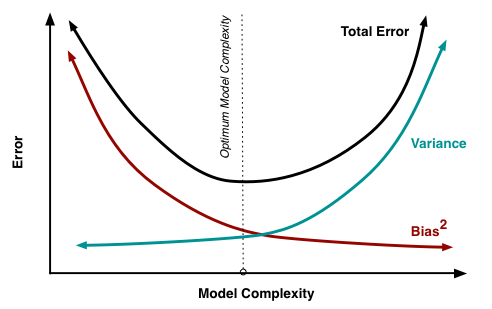
\includegraphics[height=10em]{./lectReg/biasvariance.png}\\
%\footnote{\url{http://scott.fortmann-roe.com/docs/BiasVariance.html}}
%
%\hspace{6em}
%$	\frac{dBias}{dComplexity} = -\frac{dVariance}{dComplexity}$
%\end{frame}
%***********************************************************
\begin{frame}{Finding the Sweet Spot}

\begin{columns}
\begin{column}{0.5\textwidth}

\hspace{2em}
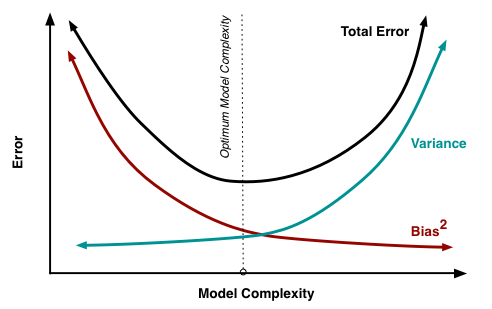
\includegraphics[height=8em]{./lectReg/biasvariance.png}

 
\hspace{6em}
$	\frac{dBias}{dComplexity} = -\frac{dVariance}{dComplexity}$
\end{column}
\begin{column}{0.5\textwidth}
\begin{itemize}
\item In practice, there's no way to measure this % no Gradient Descent
\begin{itemize}
\item Try models of different complexity
\item Choose the one with the overall lowest error
\item Relies on choice of error measurement
\end{itemize}
\end{itemize}
\end{column}
\end{columns}
\footnote{\url{http://scott.fortmann-roe.com/docs/BiasVariance.html}}
\end{frame}
%***********************************************************

\begin{frame}[fragile]{Underfitting vs. Overfitting}

\begin{table}
\begin{tabular}{ccc}
%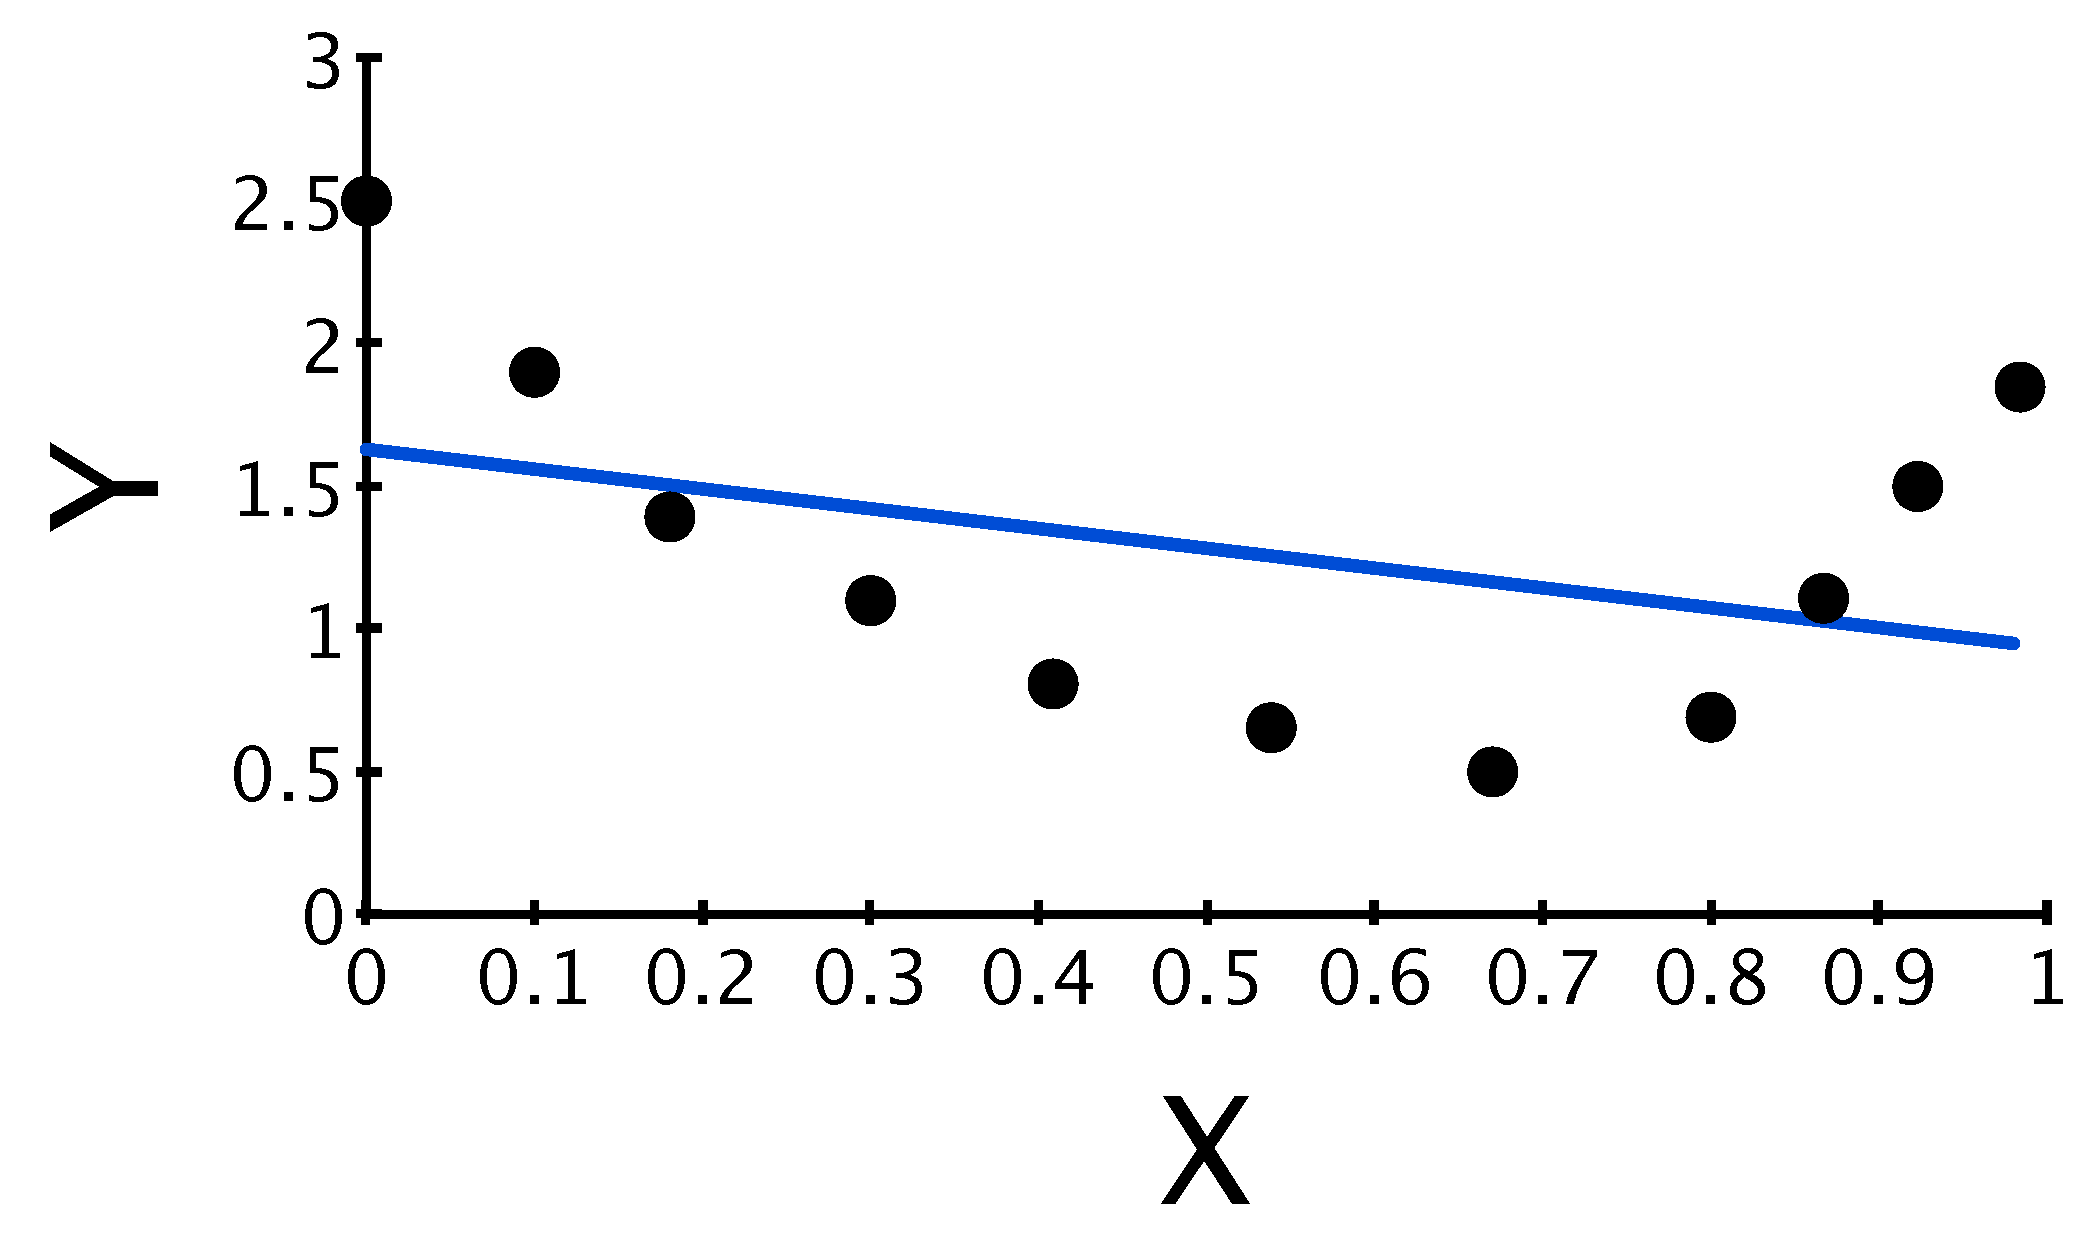
\includegraphics[height=6em]{./lectReg/OverUnderDataU1.pdf} & Complexity &}\\
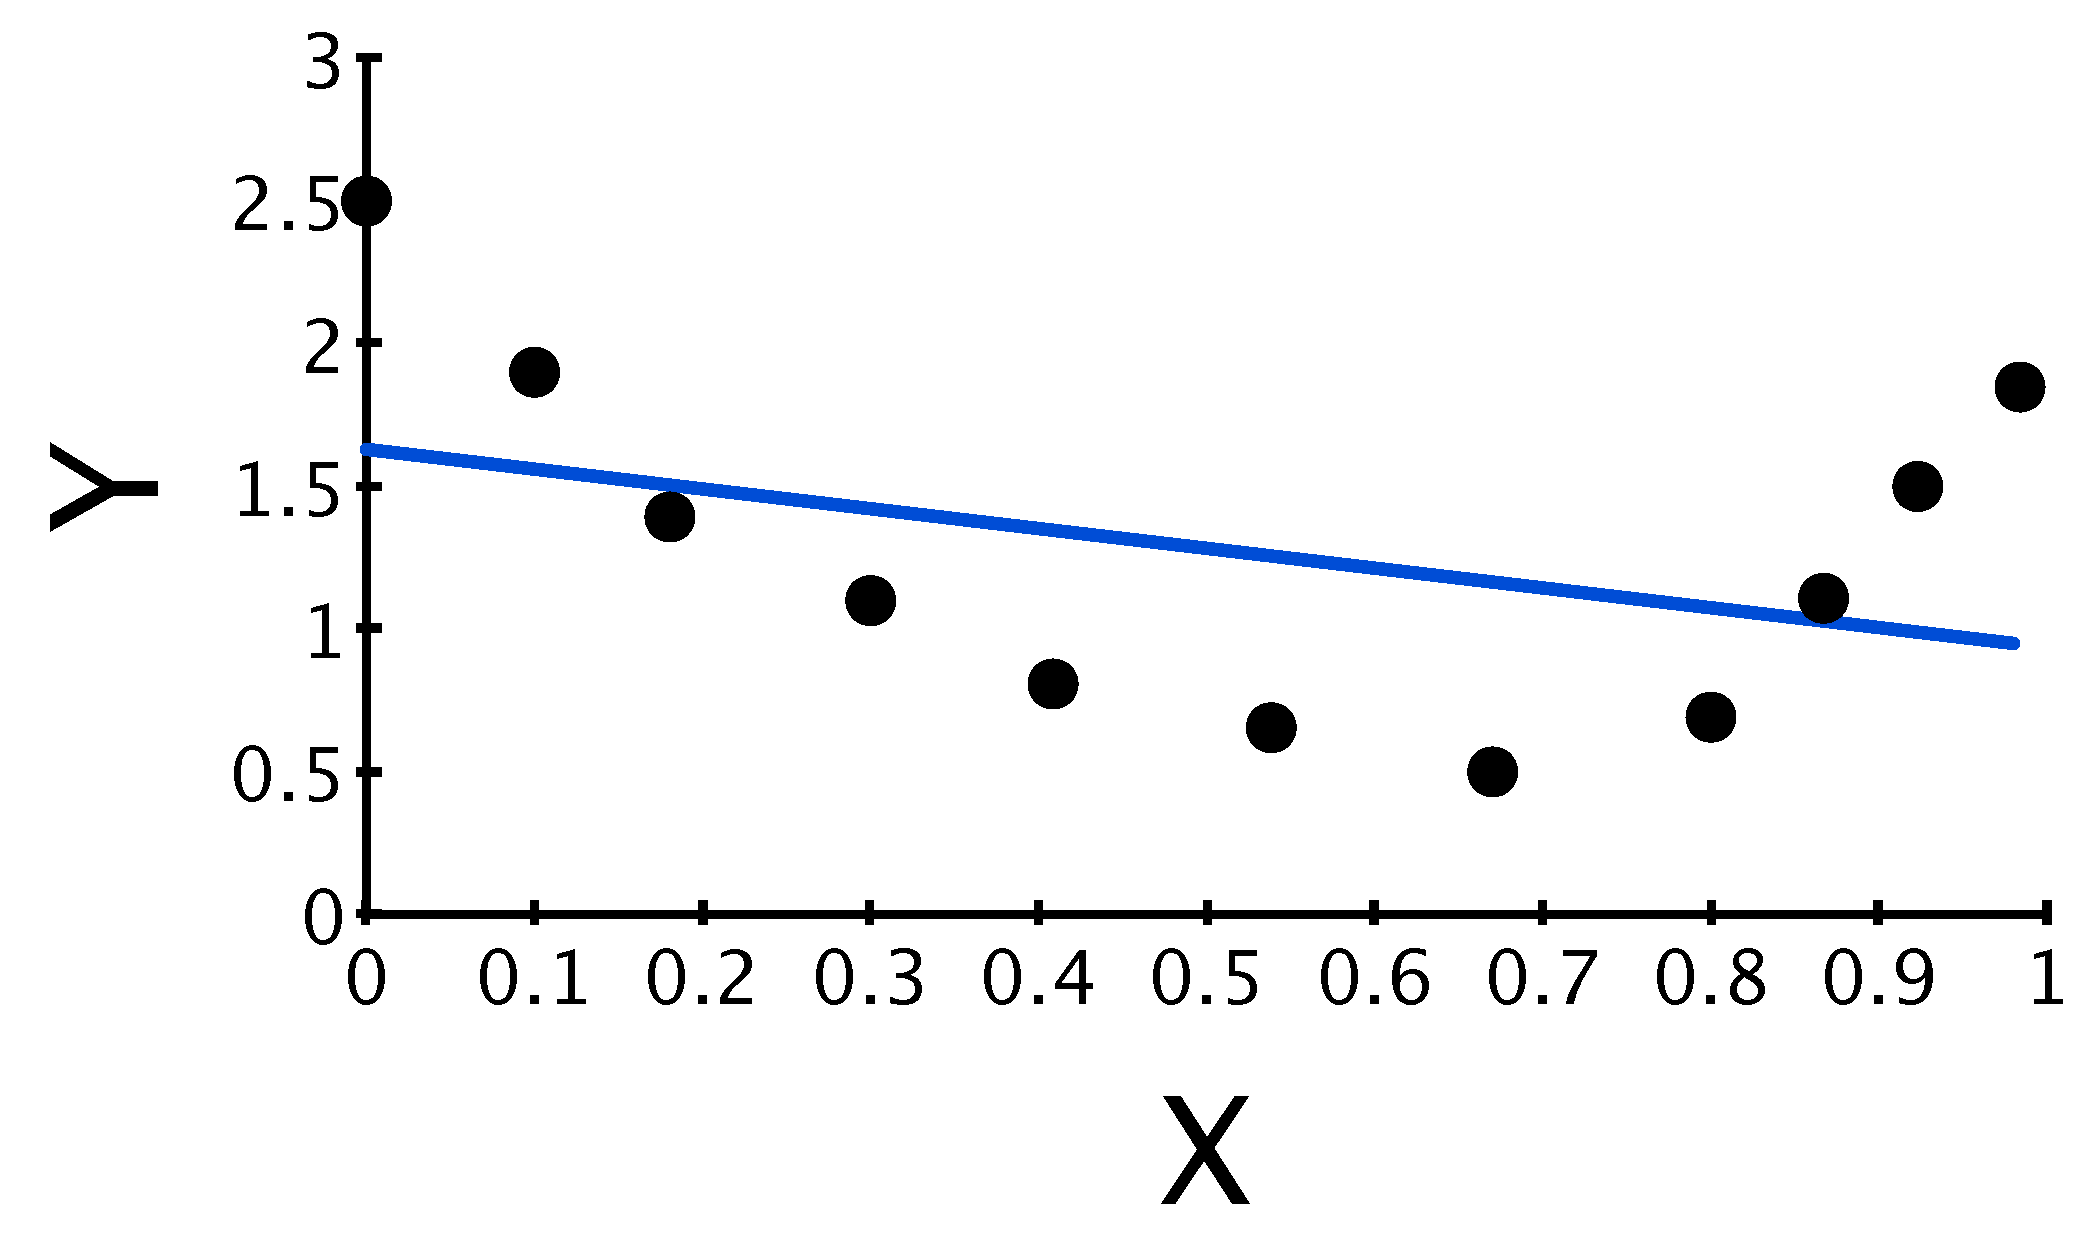
\includegraphics[height=6em]{./lectReg/OverUnderDataU1.pdf} & Complexity & 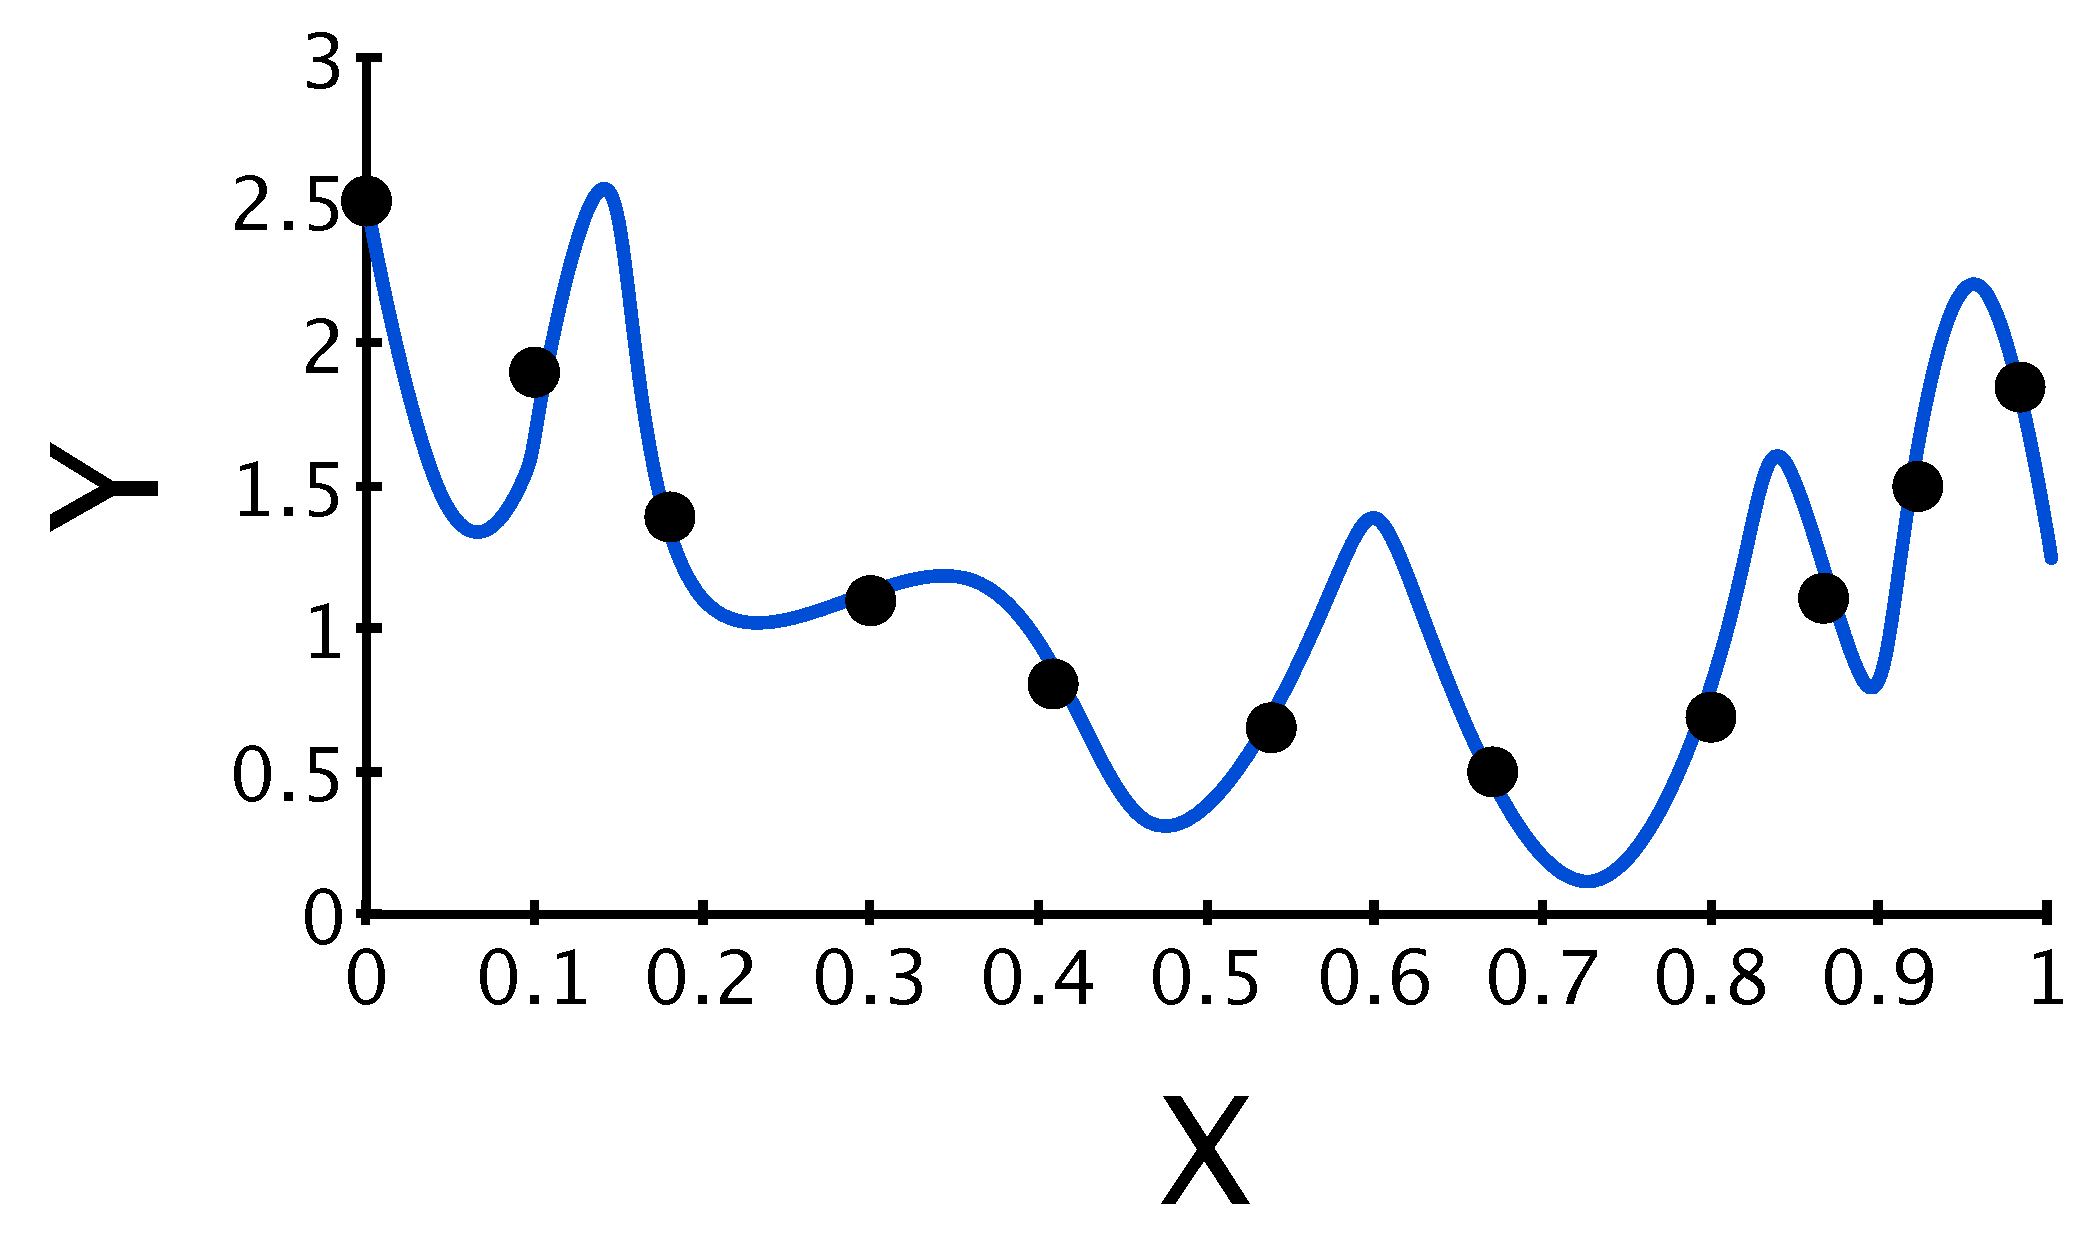
\includegraphics[height=6em]{./lectReg/OverUnderDataO1.pdf}\\
Low Complexity & $\xrightarrow{\hspace*{2cm}}$& High Complexity\\
High Bias & & Low Bias \\
Low Variance & & High Variance \\
\end{tabular}
\end{table}
\end{frame}
%***********************************************************

\begin{frame}{Regularization}

\begin{itemize}
\item One way to deal with overfitting
\item Massively important idea in data science
	\begin{itemize}
	\item In a nutshell
	\begin{itemize}
	\item Give learning algorithm ability to choose complexity of model
	\item Simpler model: lowers $Var(\hat{f}(X))$, raises inductive bias
	\item Complex model: raises $Var(\hat{f}(X))$, lowers inductive bias
	\end{itemize}
	\end{itemize}
\item Automatically choose the correct model complexity
	\begin{itemize}
	\item Balance trade-off between bias and variance
	\item To get lowest error
	\end{itemize}
\item Done by adding a penalty term to objective function
	\begin{itemize}
	\item Penalizes model for complexity
	\end{itemize}
\end{itemize}
\end{frame}

%***********************************************************

\begin{frame}{Regularization}

\begin{itemize}
\item Typically, penalty is based on $l_p$ norm
\item Recall, $l_p$ norm of a vector $\langle x_1, x_2, ... \rangle$ computed as:
$$\left(\sum_{i = 1}^n |x_i|^p \right)^{1/p}$$
\item Common penalties are $l_1$, $l_2$
\end{itemize}
\end{frame}

%***********************************************************
%
%\begin{frame}{Example: Linear Regression}
%
%\begin{itemize}
%\item Standard model form is:
%$$l = \beta_0 + \beta_1x_1 + \beta_2x_2 + \ldots + \beta_px_p + \epsilon$$
%\item Add in regularization term $\lambda \sum_i^p \
%where $\beta_i$ is the $i$th regression coefficient and  $\epsilon$ is noise
%\item Goal is the keep the values of the $\beta$s small
%\item Which reduces 
%\begin{itemize}
%\item Complexity
%\item Variance
%\end{itemize}
%\end{itemize}
%\end{frame}
%***********************************************************

\begin{frame}{Example: Logistic Regression}

\begin{itemize}
\item Standard objective function to minimize is:
$$\sum_i y_i \theta_i - \log(1 + e^{\theta_i})$$
where $\theta_i$ is $\sum_j x_{i,j} r_j$ or $X_i \cdot \boldsymbol{r}$
\item Change objective function to:
$$\sum_i \left( y_i \theta_i - \log(1 + e^{\theta_i}) - \lambda (||r||_p)^p \right)$$
% Chis uses -, that assumes maximization
$(||r||_p)^p$ is the $l_p$ norm of the regression coefficients raised to power $p$
\item We maximize the objective function, which  is why we subtract the penalty term
\item $\lambda$ is the regularization parameter
\end{itemize}
\end{frame}


%***********************************************************

\begin{frame}{Example: Logistic Regression}
	\begin{itemize}
	\item If $p = 1$ have ``the lasso''
	\item If $p = 2$ have ``ridge regression''
	\item $\lambda$ controls the magnitude of the penalty
	$$Loss = \sum_i \big( y_i \theta_i - \log(1 + e^{\theta_i})\big) + \lambda (||r||_p)^p$$
	\item As the $l_p$ norm of the regression coefficients gets bigger, the value of the Loss function increases
	\item Models with smaller norms will be preferred
	\begin{itemize}
	\item Typically, try different values of $\lambda$ during validation
	\item Usually scale $\lambda$ with $n$ 
	\item Keeps loss balanced between prediction and regularization parts as data size changes
%	\item As $\lambda$ gets small in magnitude, we get to  least squares
%	\item As $\lambda$ get larger in magnitude, we get to Ridge Regression
	\end{itemize}
\end{itemize}
\end{frame}

%***********************************************************
\begin{frame}{ Ridge Regression}
	\begin{itemize}
	\item As known as [Andrey] Tikhonov regularization
	\item Used when we want an solution to a problem that does not have a unique solution
	\item ``Ridge" local optimums
	\item Reduces coefficient values
	\item Has higher bias, but lower variance than least squares estimator
	\item $l_2$ norm (sum of squares)
	% eg $Ax = b$
\end{itemize}
\end{frame}

% least squares is unbiased, but can have high variance when features are highly correlated
% https://tamino.wordpress.com/2011/02/12/ridge-regression/
%***********************************************************
\begin{frame}{ Lasso Regression}
	\begin{itemize}
	\item \underline{L}east \underline{A}bsolute \underline{S}hrinkage and \underline{S}election \underline{O}perator
	\item Includes
	\begin{itemize}
	\item Feature selection
	\item Regularization
	\end{itemize}
	\item Credited to Robert Tibshirani 1996
	\item Designed for least squares models
	\item Primary goal to improve accuracy by:
	\begin{itemize}
	\item Reducing the number of features used in the final model
	\item This means it actually eliminates features by letting their regression coefficients be 0
	\item Forces the sum of the regression coefficients to be less than a fixed value
	\end{itemize}
	\item $l_1$ norm (sum of absolute values)
\end{itemize}
\end{frame}
%***********************************************************
\begin{frame}{Choosing between $l_1$ and $l_2$} 
%http://machinelearningspecialist.com/machine-learning-interview-questions-q8-l1-and-l2-regularization/
	\begin{itemize}
	\item $l_1$
	\begin{itemize}
	\item Can eliminate features
	\item ...at the cost of accuracy
	\item Good for 
	\begin{itemize}
		\item high dimensional data 
		\item sparse datasets (lots of features with no values)
		\item Classification
	\end{itemize}
	\end{itemize}
	\item $l_2$
	\begin{itemize}
	\item Distributes errors among the features
	\item ...often more accurate
	\item More computationally intensive
	\item Good for 
	\begin{itemize}
		\item Dense features
		\item Regression
	\end{itemize}
	\end{itemize}
	\end{itemize}
\end{frame}

%***********************************************************

\begin{frame}{Closing Remarks}

\begin{itemize}
\item When regularizing, important to normalize data
	\begin{itemize}
	\item That is, transform so mean = 0 and variance = 1
	\item[?] Why?
	\end{itemize}
%\item Bayesians argue they are protected from over-fitting
%	\begin{itemize}
%	\item A good prior protects against complex models
%	\item In fact, ``the lasso'' closely related to BLR with Laplace prior on $r$
%	\item Ridge regression closely related to BLR with Normal prior on $r$
%	\end{itemize}
\end{itemize}
\end{frame}
%***********************************************************

\begin{frame}{Closing Remarks}

\begin{itemize}
\item When regularizing, important to normalize data
	\begin{itemize}
	\item That is, transform so mean = 0 and variance = 1
	\item Why?
		\begin{itemize}
	\item In a linear model, input dims with larger values generally lead to larger outputs
	\item For a small input value to lead to a large output, it needs a large multiplier
	\item But we penalize large multipliers when regularizing
	\item To avoid bias towards dims with larger values, need to normalize
%		\item So the model doesn't have to work so hard to overcome the differences in feature magnitudes
		\end{itemize}
	\end{itemize}
%\item Bayesians argue they are protected from over-fitting
%	\begin{itemize}
%	\item A good prior protects against complex models
%	\item In fact, ``the lasso'' closely related to BLR with Laplace prior on $r$
%	\item Ridge regression closely related to BLR with Normal prior on $r$
%	\end{itemize}
\end{itemize}
\end{frame}
%***********************************************************
\begin{frame}{Questions?}
\begin{itemize}
	\item What do we know now that we didn't know before?
	\vspace{5 em}
	\item How can we use what we learned today?
\end{itemize}
\end{frame}


%References
%\begin{enumerate}
%\item https://ml.berkeley.edu/blog/2017/07/13/tutorial-4/
%\item http://scott.fortmann-roe.com/docs/BiasVariance.html
%\item https://elitedatascience.com/bias-variance-tradeoff
%\end{enumerate}



\end{document}
